\part{The Robot Coworker} % Main chapter title

\label{part:robot_coworker} % Change X to a consecutive number; for referencing this chapter elsewhere, use \ref{ChapterX}

\lhead{Part 2. \emph{The Robot Coworker}} % Change X to a consecutive number; this is for the header on each page - perhaps a

Robots can be used to perform a large number of different operations. Some of these will be simple enough that the robot can just achieve its task by performing a prefixed sequence of elementary actions. In other cases, the robot might have to achieve complex goals, which require the ability to create plans and to adapt them to the current state of the world. When cooperating with other agents, the robot has to build a shared plan, which includes the actions that every agent need to perform, in order to coordinate and ensure the corrent achievement of the goal. We can imagine the following process:
\begin{itemize}
	\item The system receives a new goal. This can be directly introduced by a human, or chosen after some kind of reasoning by the robot.
	\item One of the agents (the robot or the humans) proposes a plan to achieve the goal, and presents it to the other agents.
	\item The agents negotiate the plan. In some situations, one of the agents might not be able (or might not want) to perform a specific action, or sequence of actions. The agent can refuse the plan, proposing a correction or a completely different plan.
	\item The agents execute the plan. Each agent performs its part of the plan. In addition, agents may check the state of others to monitor the correct execution of their part of the plan or to cordinate with them.
	\item An agent might fail its part of the plan. If this happens the agents need to create a new plan to account for this failure.
 	\item The process continues until the goal is achieved or it becomes unachievable (for example, a needed resource is no longer available).
\end{itemize}

When humans cooperate this process can be very quick. For simple tasks humans are able to coordinate without explicitly forming a plan, in particular if they are used to cooperating together. Other times, when there are unexpected problems during the execution of a plan, humans are able to quickly readapt their plan, without completely restarting this process. In order to cooperate in a natural way with humans, robots need to reproduce these mechanisms.

In this part we will introduce the mechanisms that we developed for the robot coworker problem. In this problem, the robot has to achieve a goal together with a human, cooperating to solve the task. The main aspects of our works are the management of plans, shown in chapter~\ref{chapter:plan_management}, and their execution, particularly the execution of joint actions, shown in chapter ~\ref{chapter-task_execution}. Chapter ~\ref{chapter-coworker_experiments} shows our experiments in robot coworker problem. We also show, in chapter ~\ref{chapter-madp} a recent extension to this work, involving multi-agent probabilistic planning.

% Chapter Template

\chapter{Plan Management} % Main chapter title

\label{chapter:plan_management} % Change X to a consecutive number; for referencing this chapter elsewhere, use \ref{ChapterX}

\lhead{Chapter 6. \emph{Plan Management}} % Change X to a consecutive number; this is for the header on each page - perhaps a shortened title

In this chapter, we introduce the Plan Management capacity of our system. Section~\ref{sec:plan_management-intro} introduces the subject, with a review of two systems able to manage cooperative plans. Section~\ref{sec:plan_management-overview} shows the main aspects of this component. Our system is able to use different plan management modalities, as explained in section~\ref{sec:plan_management-modalities}. Section~\ref{sec:plan_management-hatp} introduces HATP, a human-aware multi-agent planner interfaced with our system. Section~\ref{sec:plan_management-plan_manager} introduces our algorithm to manage plans. Finally, section~\ref{sec:plan_management-plan_monitoring} explains how we compare human activities with the current cooperative plan.

\section{Introduction}
\label{sec:plan_management-intro}

When agents cooperate, they agree on a common plan to solve the task, implicitly or explicitly. We call this sort of plan a \textit{shared plan}.  Participants in a shared plan do not limit themselves to simply execute their parts of the plan, but, in fact, need to constantly monitor other participants, to synchronize their actions and adapt their plans to them. Let us an imagine a situation where the robot is executing a shared plan with Greg. If the robot execute its own actions without observing Greg we might encounter several situation where the two will put in danger, perhaps even preclude, the achievement of the goal. For example, Greg might be late in executing a crucial action, and the robot should wait for him. An even more dangerous example happens if Greg has starts following another plan, for personal choice or for other circumstances, and does not inform the robot about this change. If the robot does not notice that Greg has changed his strategy, and does not adapt its own plan, the two might not be able to achieve their goal.

We call \textit{plan management} the process where the robot executes its own actions while coordinating with others and monitoring their activities. 

Two examples of systems able to execute shared plans are  Chaski \citep{shah2011improved} and Pike \citep{levine2014concurrent,karpas2015robust}.

Chaski is an executive system that enables the robot to anticipate and adapt to other agents actions. Chaski is based on human teamwork strategies, including ideas such as least moment commitment, frequent communications on the task status, and considering the consequences of the robot's choices on other agents. Chaski is able to execute plans in two different modalities: Equal Partners and Leader and Assistant. The system receives as input a shared plan, which includes the activities that need to be performed, the capacities of each agent, and the deadlines for these activities. Chaski produces a compact representation of all the possible schedulings of activities, based on this plan, which is used to take decisions on the fly during execution and to adapt to human choices. Results show that Chaski is able to reduce human's idle time in an equal partners scenario. A possible problem of this approach is that, if an agent completely deviates from the chosen plan, the system needs to create a new plan, which needs to be encoded again.

Pike is another executive, able to simultaneously recognize human plans and adapt to them. Pike receives as input a plan, represented as a Temporal Plan Network with Uncertainty (TPNU). Pike represents this plan by considering controllable choices (i.e. actions) for the robot and uncontrollable choices for the human. The idea is considering that these choices are not independent.  In this way the system can infer what actions the human would rationally take to achieve his goal and what actions the robot should take to help him. The system receives a stream of human choices, which allows it to determine the robot's actions. Pike has been tested in simulation and with a real robot with good results, managing, on average, to take decisions with a low latency.

If the human does not follow the TPNU Pike will return a failure. The authors discuss integrating the system with a generative planner in the future to overcome this limitation.

In the next sections, we will present our approach to the problem.

\section{Overview}
\label{sec:plan_management-overview}

\subsection{Process Overview}
Our Plan Management module receives, as input, a goal, which can be generated by the system or introduced by a human, using a tablet interface. After receiving a goal, the system will request a multi-agent plan to the task planner, including the actions of the robot and of other humans. We do not deal, in this module, with issues of task scheduling, which we leave to the task planner. While, in this chapter, we will concentrate on cooperative plans, our system is completely able to manage plans with only one agent, robot or human. 

One of the goals of our system is flexibility; we consider important the possibility to interface with external components. Different planners can interface with our plan management algorithm, if they respect our interface.

For each scenario, we define a planning \textit{domain}, which includes every entity and task that can be used in plans for that scenario. We consider that plans can be decomposed in a set of sub-parts, that we call \textit{tasks}. In general tasks can be further decomposed in simpler sub-tasks, until reaching the most basic form of task of a domain, which we call \textit{action}. Both actions and tasks follow the same representations, $(name,preconditions,target,postconditions)$, that we introduced in chapter~\ref{chapter:belief_management}. In chapter~\ref{chapter:intention} we introduced our intention and action recognition module. As we said, this this module possesses a list of known actions. Every action in a planning domain that can be performed by humans need to be present in this list. In this way, the system will be able to monitor the execution of actions by humans, by using the mechanisms of the robot observes. This process will be explained in more details in section~\ref{sec:plan_management-plan_monitoring}.

In some situations, to be more generic, we will use the word \textit{task} to refer to both tasks and actions, since actions are actually tasks that can not be decomposed in the current planning model.

Each planner used by our system needs to represent its plans as a set of streams, one for each agent. A stream is a sequence of nodes, where each node corresponds to task assigned to be executed by the agent. Nodes can be connected by causal links, even among different streams, to ensure synchronization. A causal link $l=(t_1,t_2)$ indicates that  task $t_1$ should be execute before task $t_2$. This ensures that all the preconditions to execute $t_2$ are fulfilled. Moreover, if $t_1$ and $t_2$ are executed by different agents, and if there is a shared resource connected to the task, the causal link indicates that the resource will be released by the agent only after $t_1$ is completed. An example of this data structure is shown in figure~\ref{fig:plan_management-streams}.

\begin{figure}[ht!]
 \centering
  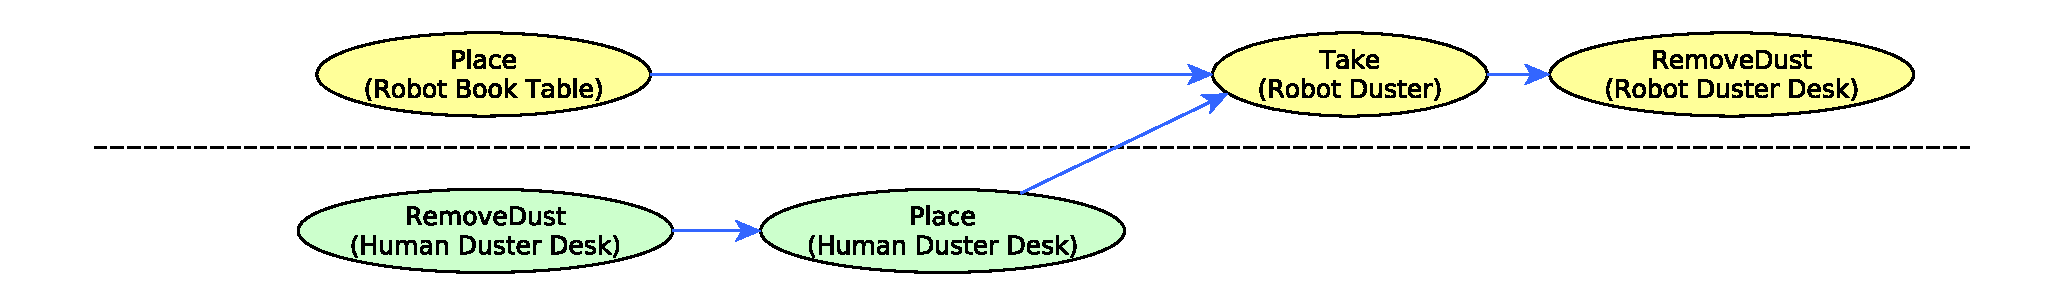
\includegraphics[scale=0.45]{img/coworker/plan_management/streams.pdf}
 \caption[Plan data structures]{
 A plan stream structure. The upper stream represents the robot, and the lower one a human. Each node represents a task to be performed by the agent. For each task, the stream shows its name and, in parenthesis, the name of the agent and the parameters of the task. Causal links are represented as arrows between the nodes. Notice the causal link between the Place(Human Duster Desk) node in the human stream and the Take(Robot Duster) node in the robot stream. This link indicates that the robot should wait that the human places the duster before executing the action to take it, ensuring synchronization.}
 \label{fig:plan_management-streams}
 \end{figure}

The system will manage each stream separately. By using the causal links, the robot is able to synchronize with humans. Joint actions (e.g. cooperative actions executed by two agents) will be treated by this module as actions of the robot, and be executed with a specific framework,  explained in chapter~\ref{chapter:task_execution}.

Plans can be managed in three different modalities. The robot can be the leader, choosing a plan and guiding the human in its execution. The robot can also be an assistant, and follow the orders of the human. Finally, the robot and the human can be equal partners. This mechanisms will be explained in section~\ref{sec:plan_management-modalities}.


% \begin{itemize}
% 	\item Interface with external planners in order to create a shared plan. The system has been integrated with a HTN (Hierarchical Task Network) based planner, HATP (Human-Aware Task Planner), and with a multi-agent MDP planner.
% 	\item Monitor a human plan. Our system is able to monitor other agents' parts of a plan, to cordinate with them and to react when an agent fails an action or his actions diverge from the current plan.
% 	\item Receive plans from a user. Users can interact with the robot with a tablet application, asking it to execute specific actions or goals.
% 	\item Executing shared plans in different modalities. The robot can be a leader, assistant, or equal partner of humans during plan management.
% \end{itemize}

\subsection{Architecture}
A number of modules implement these ideas, as shown in figure \ref{fig:plan_management-architecture}:
\begin{itemize}
\item Task Planner. Creates a shared plan for the involved agents. We consider the Task Planner as an external module. Our system has been integrated with the HATP planner, which we will introduce in section~\ref{sec:plan_management-hatp}. We have also recently introduced a probabilistic multi-agent planner based on MDPs, which we will discuss in chapter~\ref{chapter:mamdp}.
\item Plan Manager. Manages the current plan, interacting with the Task Execution layer to execute the robot's tasks and with the Situation Assessment layer to monitor humans' tasks.
\end{itemize}

After receiving a goal from the Goal Management layer, the Plan Manager module sends a request to the Task Planner to look for a suitable plan. After receiving a plan, this module will interact with the Task Execution and Situation Assessment layers to execute it. 

\afterpage{\clearpage}
\begin{sidewaysfigure}[ht!]
	\centering
	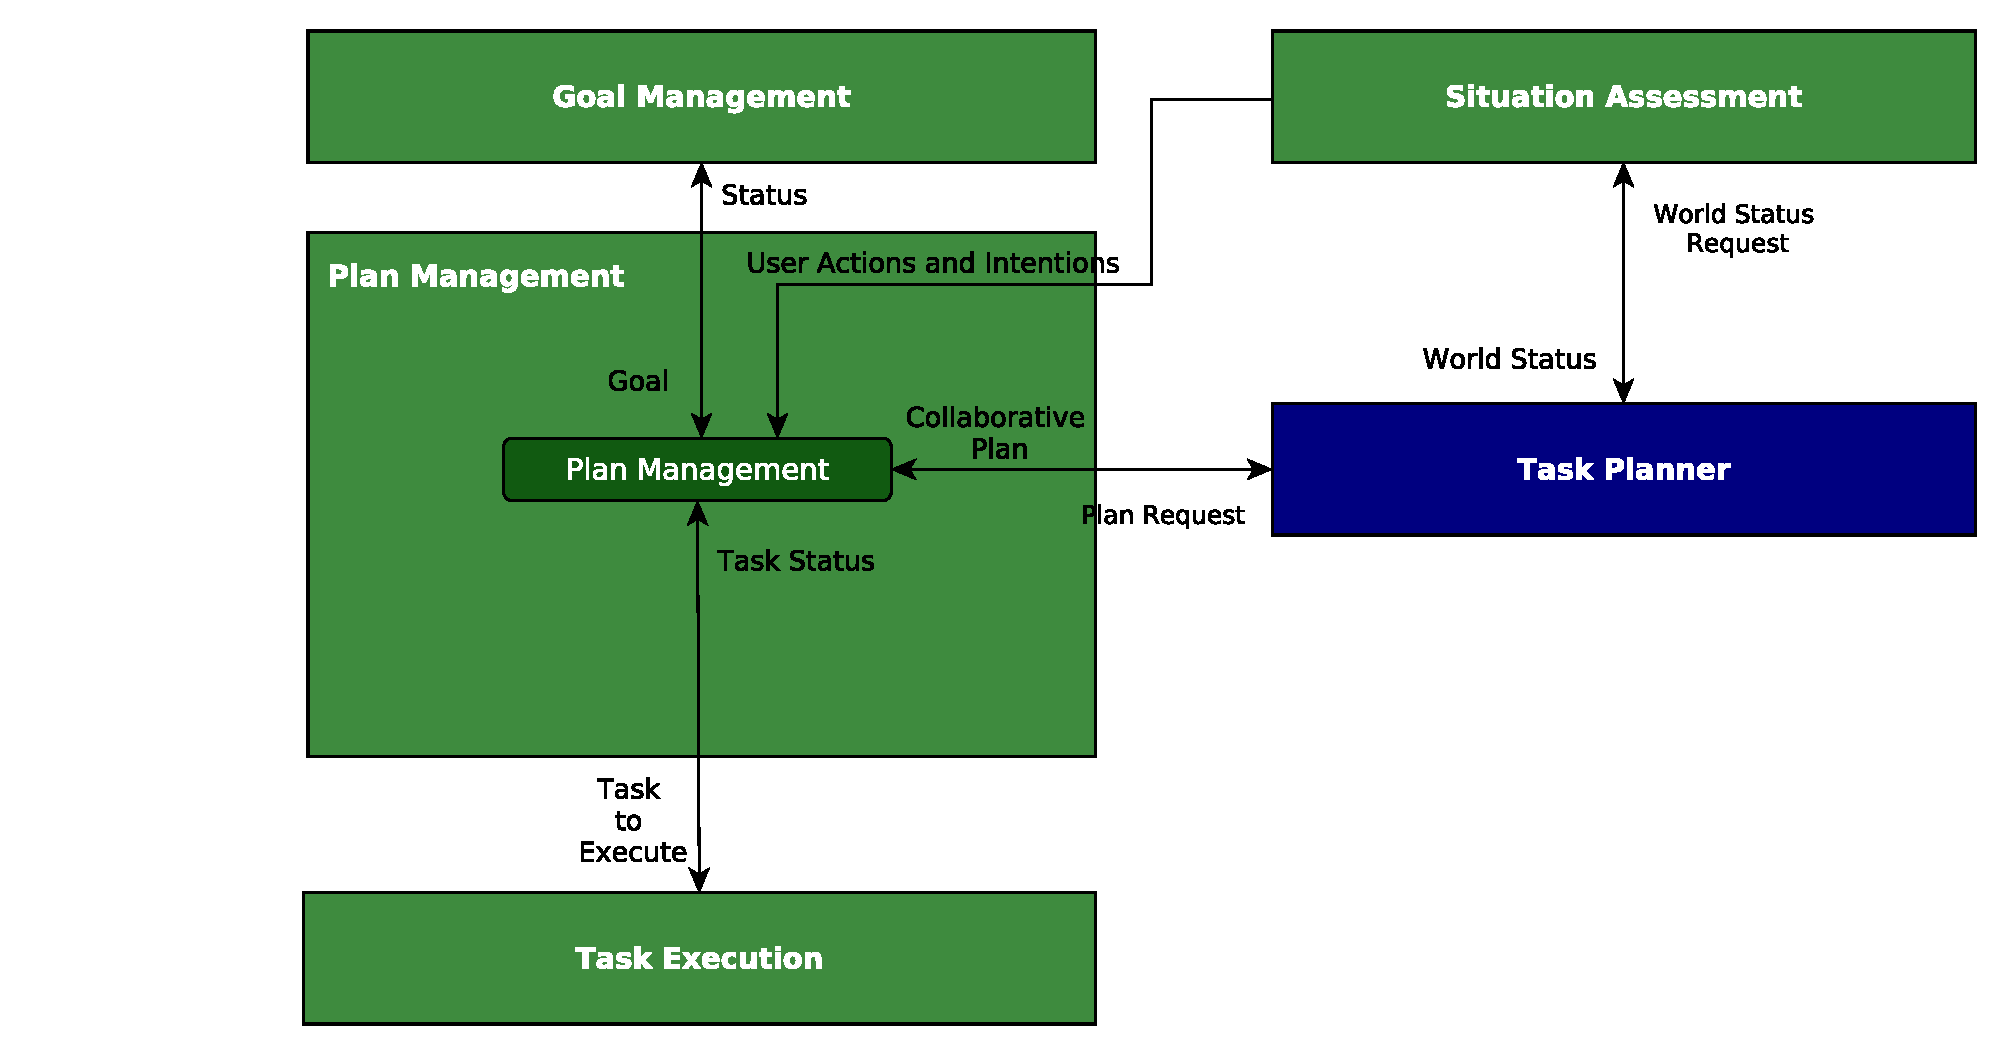
\includegraphics[scale=0.5]{img/coworker/plan_management/plan_management_architecture.pdf}
	\caption[The architecture of the Plan Management layer]{The architecture of the Plan Management layer. Light green rectangles represent modules, while dark green rectangles layers. The Task Planner is shown as a blue rectangle to indicate that it is a module external to the system. Arrows represent messages exchanged between components, with the label detailing the message.}
	\label{fig:plan_management-architecture}
\end{sidewaysfigure}


Parts of this chapter were presented in \cite{Lallement2014,fioreiser2014}.

\section{Plan Management Modalities}
\label{sec:plan_management-modalities}
When acting together, agents sometimes do not have the same decision power, with one of them assuming the role of a leader. We represent this idea, in our system, by proposing three different modalities: \textit{robot leader}, \textit{human leader}, and \textit{equal partners}. The robot is able to switch from one modality to another during the execution of a plan. For example, if the current modality is \textit{robot leader} and the Robot receives a command from a user, it will switch to the \textit{human leader} modality, after interrupting its current action.

\subsection{Robot leader}
\label{subsec:plan_management-robot_leader}
In this modality the robot, after computing the plan, will present it to the user and start executing it. The robot will track the status of humans, informing them of which actions they should execute. This modality can be helpful when interacting with  naive users or in tasks where the robot has a better knowledge of the  domain or of the environment than the other agents.

We have developed two different algorithms to present the computed plan to the user. In the first, simpler case, the robot will verbalize sequentially all the actions, stating which agent should perform them. 

For example, the plan presented in figure~\ref{fig:plan_management-streams} would be explained in the following way: ``I will place the book on the table. You will remove the dust from the desk and then place the duster on the desk. After that, I will take the duster and then I will remove the dust from the desk".

To generate this kind of verbalization we create a textual representation for each object and task, and then verbalize it with a text-to-speech application. Using simple rules, we follow the plan streams and verbalize each node. To create a more interesting and varied explanation, we use some connective words between nodes. We added some randomness in the algorithm. For example, the robot will randomly select words such as ``At this point", ``After that", or ``Then" to introduce a task. Since this algorithm is not a focus of our work we will not present it in details.

 We have also developed a more advanced algorithm to adapt this process to the expertise of a user in the tasks to execute. We will present this algorithm in chapter~\ref{chapter:knowledge}.

\subsection{Human Leader}
The human can also create plans, interacting with the robot by using a
tablet application, shown in figure~\ref{fig:plan_management-tablet}. Using the tablet, the human can choose a goal for the robot, but also pause or stop its actions. The human can choose, as goal,  the execution of a simple action, but also of a more complex task, involving many actions.


In this modality the robot  will simply observe the surroundings and wait for user inputs. User commands have a priority over the other two plan management modalities. If the robot receives a command from the
application while it is in another modality, it will abandon its current
plan, stopping its actions at a safe point, and then execute the user's
command. 

We feel that this interaction modality is important for two
different reasons.  First, some users will simply prefer to be in
charge of the execution process, for a matter of personal preference or because they
feel they have a deeper knowledge on how to realize the current task
than the robot. We can picture, for example, industrial or medical
scenarios, where the human is the leader and asks the robot to perform
different tasks to help him, when needed.

 A second use of this modality is in situations where
the robot does not have  a clear estimation of the users' intentions and
goals. For example, in a domestic environment, a user could decide to
order a robot to bring him a drink, a need that the robot can not always anticipate.

\begin{figure}[ht!]
 \centering
 \includegraphics[scale=0.25]{img/coworker/plan_management/tablet.pdf}
 \caption[Giving goals to the robot]{The human is giving a goal to the robot by using a tablet application.}
 \label{fig:plan_management-tablet}
 \end{figure}

\subsection{Equal Partners}
In the last presented operation modality the robot will try to help
the human to complete a task. At the start of the scenario, the robot
will observe the environment. After the user takes an
action the robot will calculate a plan and try to help as it can, by
performing actions related to that task and by giving helpful information to
the user, for example to fill gaps in their knowledge. In this modality, 
the robot will not explain or negotiate the current plan and will not warn humans if
their actions differ from the plan computed by the robot.

We feel that, particularly in non-critical tasks, where defining an accurate plan between the partners is not
fundamental, this modality is a very natural way of
interaction between different partners.



\section{Human-Aware Task Planner}
\label{sec:plan_management-hatp}
In this section we will briefly introduce HATP~\citep{Lallement2014}, a planning framework that we used in many experiments with our system.

Computing a plan in complex environments can be very hard and time consuming. A useful approach to reduce the search space in planning is introducing the knowledge of an expert in the system, in order to guide the planner toward desirable states. An implementation of this idea is Hierarchic Task Network (HTN), where the domain expert specifies a hierarchical library of operations, called methods, when the operation is a node in the hierarchy, and actions, when the operation is a leaf. HATP extends HTN for human-robot interaction problems. Among the capacities of HATP we can find:
\begin{itemize}
\item Multi-Agent. HATP is able to include different agents in its domain, specifying which actions each one can execute. HATP is able to plan for different agents at the same time, humans and robots. The planner can also compute ``joint actions", that involves more agents at the same time.
\item Social Rules. The domain expert can introduce a set of rules, which represent desirable behaviors. Social rules help producing human-aware plans, that avoid behaviors that can be considered rude for humans. Using social rules, HATP can also balance in different ways the amount of effort of each agent in the plan. For example, we might choose that the human should have a minimum effort in the plan, or that the effort should be balanced between the human and the robot.
\item Cost Driven. The domain expert can specify a cost for actions. Plan pruning allows to explore more efficiently the search space, discarding paths that are not promising.
\end{itemize} 

Plans are represented as an HTN tree decomposition and as a set of streams, one per agent, which shows which actions each agent needs to perform. Causal links are introduced between streams to ensure synchronization.

\section{Plan Management}
\label{sec:plan_management-plan_manager}

Our plan management algorithm receives as input a plan composed by a set of streams, one for each agent. Each stream will be handled in parallel, using different threads of execution. We will now explain this algorithm, which is shown in figure \ref{fig:plan_management-manage_plan}.
\begin{itemize}
  \item Each thread executes the part of the plan of an agent, composed by $n$ different tasks.
  \item For each task, for every causal link $(t_i,t_n$), where $t_n$ is the current task, and $t_i$ is another task, the plan manager waits until $t_i$ is completed, or there is an error. This process is handled in the \textit{waitCausalLinks} procedure.
  \item When all the causal links have been satisfied, the execute\textbackslash monitor procedure is called, depending if the thread is managing the robot or a human. The \textit{executeTask} operation interacts with the Task Execution layer to complete the task, while the MonitorTask operation with the Situation Assessment layer.
  \item If these procedures succeed, the Plan Manager switches to the next task, otherwise it returns a failure.
  \item The process is continued until there is a failure or the plan for the current agent is completed.
\end{itemize} 

\begin{figure}[ht!]
 \centering
 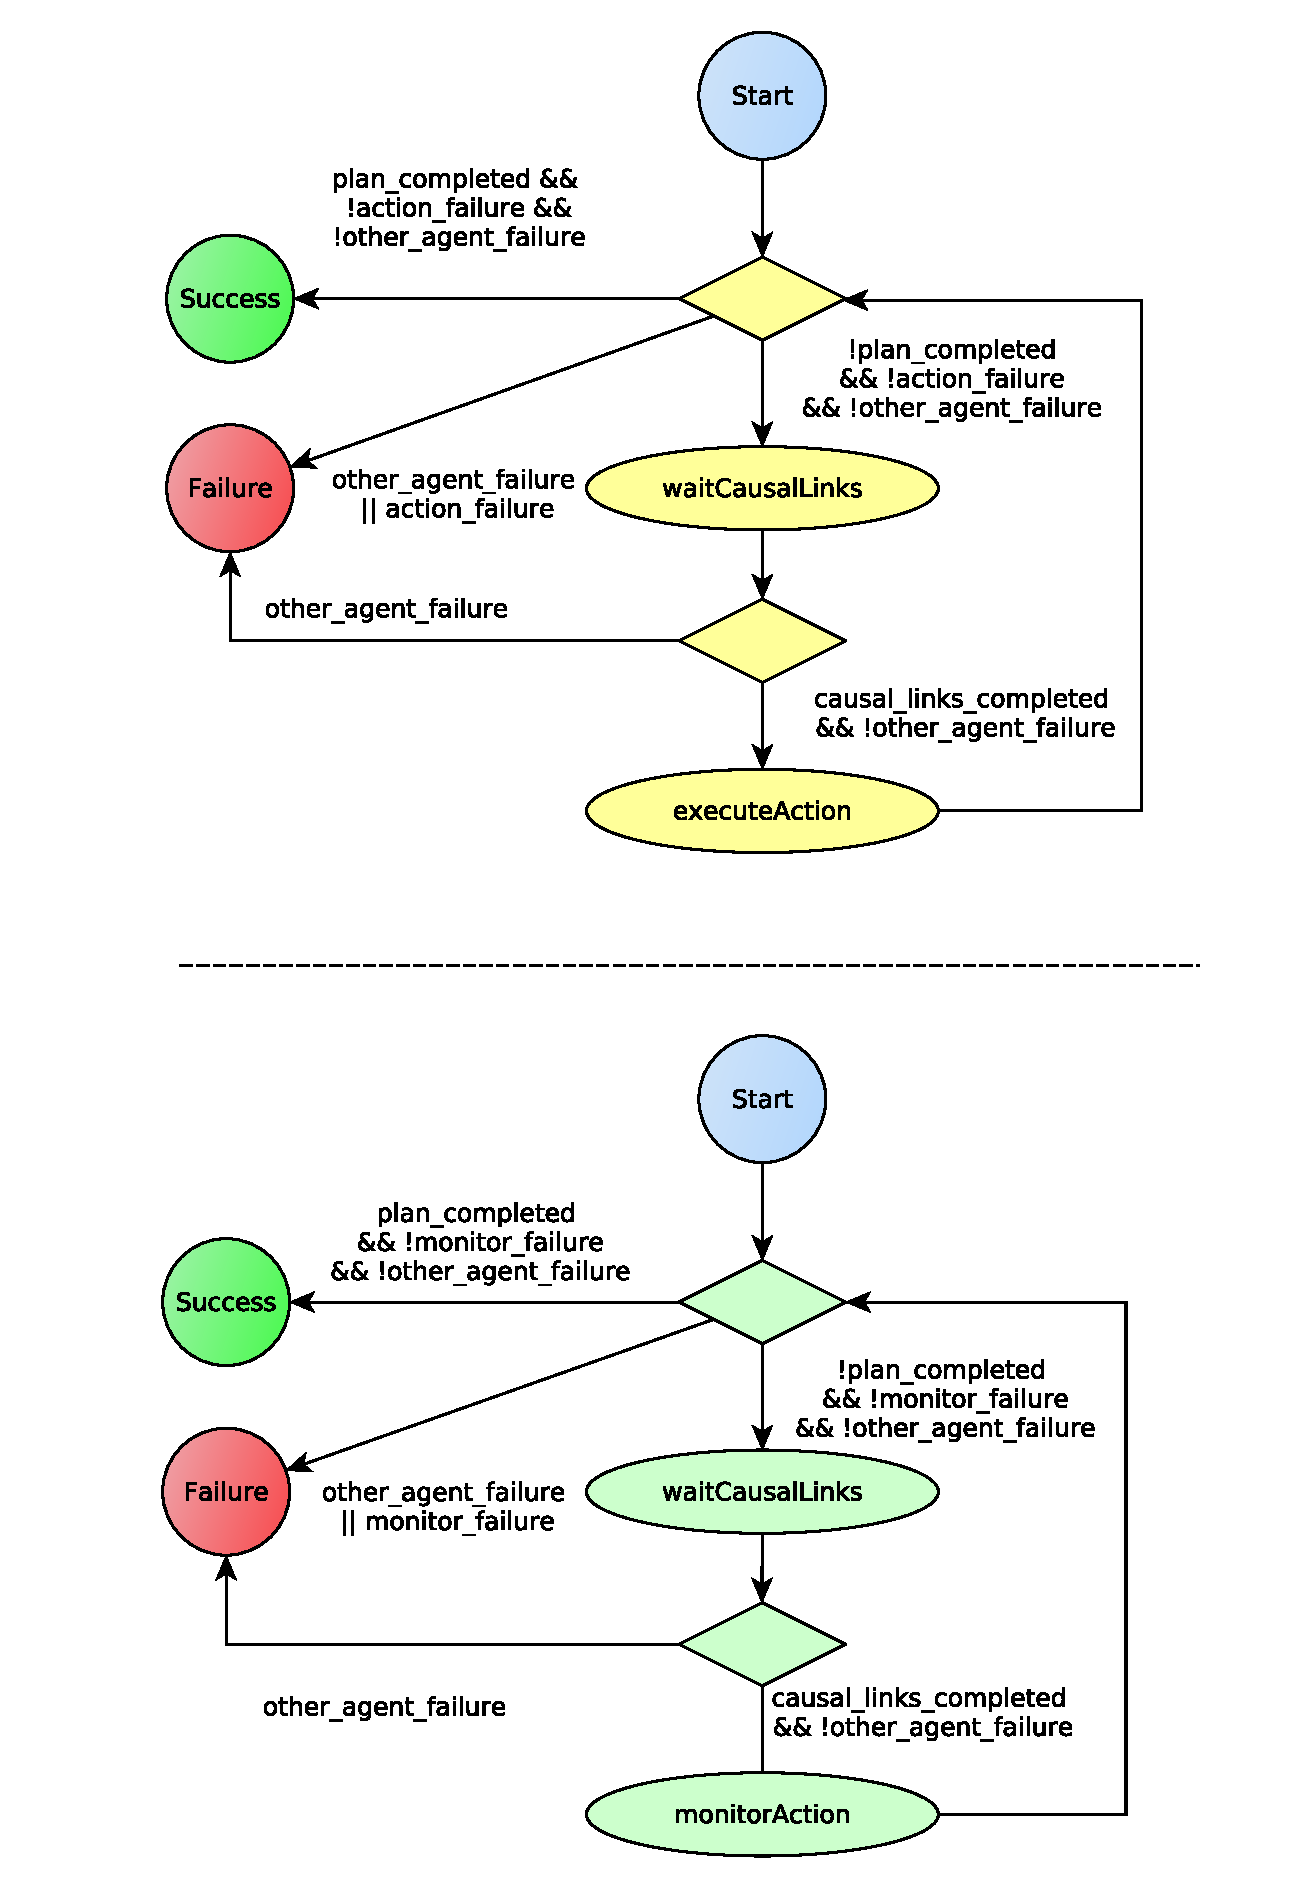
\includegraphics[scale=0.6]{img/coworker/plan_management/manage_plan.pdf}
 \caption[Plan Management Algorithm]{The plan management algorithm. The algorithm is composed by different threads, one for each agent. In this instance, the upper lane represents the robot's management thread, while the bottom a human's management thread. Elliptic nodes represent operations. Diamond nodes, representing divergences in the algorithm, where added to the graph only when they could simplify the understanding of the algorithm. Arrows imply a transition between nodes, with the label of the arrow representing the condition of the transition, when present. The absence of a label implies that a transition is always applied. The blue circle node, called ``start", represents the start of the algorithm. The green and red circle nodes, instead, represent the success or failure of the algorithm.}
 \label{fig:plan_management-manage_plan}
 \end{figure}

Failures in the algorithm lead to a replan request. If a new plan is found, the algorithm starts again, otherwise the goal is considered as failed. Depending on the modality, the robot will also give different verbal information to the human.

If the current management modality is \textit{robot leader}, the robot will warn the human the he executed a wrong action. If the replan is successful, the robot will explain the new plan to the human. 

When the human is the leader, the robot is following orders. The current order might be to execute a task which still requires coordination, and the robot might expect the human to follow a particular strategy. If the human deviates from this strategy the robot will replan, but not issue any warning.

A similar approach is used in the \textit{equal partners} modality. In this case, the robot will adapt to the deviations in the humans' actions, but the replanning process should be almost hidden from the human, in order to be more natural. The robot will replan and start managing the new plan without informing the human.

% In this modality, the robot will expect users to execute a specific set of tasks, warning them if they do not respect this allocation. Sometimes, the robot will choose the decomposition of the tasks that should be executed by a user, but, when the partner is competent enough in a high-level task,  we may want to allow him the flexibility to execute it as he sees fit. 

\section{Task Monitoring}
\label{sec:plan_management-plan_monitoring}

During the execution of a plan, the robot will monitor other human partners. In general, having a shared plan, the robot knows what is the next task that the human should perform, and can monitor if it is accomplished. Task monitoring poses a number of different issues:
\begin{itemize}
\item Understanding when the next expected action has been performed. In some situations the robot will monitor the execution of a specific action. In this event, it needs to understand when the action has been completed.
\item Understanding when the next expected task has been performed. In some situations, the robot wants to give a human cooperator the freedom to perform a task (that is, a complex operation that can be composed by a sequence of actions) as he sees fit. This is a more complex problem than monitoring a specific action, since the robot needs to reason on the results of sequences of actions.
\item Evaluating the human engagement in the current task. The robot needs to understand if the human is trying to accomplish its current task, if he momentarily interrupted it, or if he abandoned it.
\end{itemize}

At the moment, we have implemented and integrated in our system only monitoring of actions. We will show how we include this idea, and then illustrate in the chapter~\ref{chapter:mamdp} how we could extend our system to monitor tasks and evaluate the human engagement in the current task.

\subsection{Monitoring Actions}
At all time, as previously explained in chapter~\ref{chapter:intention}, the robot constantly observes the environment, monitoring which actions are executed. As previously said, each action that can be executed by a human needs to have the same representation in the Situation Assessment and Plan Management layers. When the Plan Manager needs to monitor an action $a$ of a human stream, its $preconditions$ will be satisfied (since, if we are monitoring $a$, all of its causal links have been already satisfied). This means that $a$ will be present in the IG for the human, which will be monitoring its execution (chapter~\ref{chapter:intention} gives more details about this mechanism).

As we said in section~\ref{subsec:intention-unknown_intentions}, the single-agent MDP mechanism that we introduced is not sufficient to monitor a joint goal, and so the IG for the human, in the coworker scenario, only includes Actions and Observation nodes.

The Plan Manager will wait for Situation Assessment to infer that an action has been performed by the human. If the action is different from $a$, it will return an error, prompting a replan. Otherwise, the plan management will continue with the next action in the stream, if there are any.

For example, let us imagine a scenario where Greg is near a table, with a \textit{bottle} and a \textit{book} on top. Let us say that, at the moment, Greg can execute three actions: \textit{take book}, \textit{take bottle}, and \textit{move kitchen}. The current IG for Greg will include these actions, as well as observations to infer their execution. In this example, Greg's plan is represented by a stream of three sequential actions: \textit{move to table, take bottle, move kitchen}. 
Greg has just completed the action \textit{move to table}, and should now execute the action \textit{take bottle}, if he follows this stream. If the system infers that Greg executes \textit{take book} or \textit{move kitchen}, the plan manager will replan, since Greg executed a different action that the one that was expected. If Greg executes \textit{take book}, the system will start monitoring the next action in the stream, which is \textit{move kitchen}.


\subsection{Monitoring and Unseen Actions}
Often, in cooperative tasks, agents will operate in different locations, and so they can not observe each other actions all the time. Perhaps one of the agents is cooking in the kitchen,  while the robot is preparing the table for dinner. While we do not deal, in this work, with these issues, there are several studies on plan recognition in partially observable environments, like \cite{geib2005partial}. 
% Chapter Template

\chapter{Task Execution} % Main chapter title

\label{chapter:task_execution} % Change X to a consecutive number; for referencing this chapter elsewhere, use \ref{ChapterX}

\lhead{Chapter 7. \emph{Task Execution}} % Change X to a consecutive number; this is for the header on each page - perhaps a shortened title

This chapter shows how our system is able to execute tasks, and particularly joint actions. Section~\ref{sec:task_execution-intro} introduces the subject. Section~\ref{sec:task_execution-overview} describes our approach and the components that implement it. Section~\ref{sec:task_execution-action_executor} shows the main aspects of the Task Executor module, while section~\ref{sec:task_execution-collaborative_planners} introduces the framework we use to execute human-robot joint actions, the Collaborative Planners. Finally, section~\ref{sec:task_execution-handover} shows an example of a Collaborative Planner for human-robot handovers.


\section{Introduction}
\label{sec:task_execution-intro}
Acting in a human-crowded environment is a difficult problem. Even when acting independently, the robot needs: to ensure human safety, by taking others into account when planning and stopping if its actions could bring harm to them; to perform legible movements, so that its actions can be understood by humans (studied, for example, in~\cite{dragan2013legibility}); and to be robust, trying to complete its tasks even in front of unexpected conditions. 

These issues show us that humans should not be treated as simple obstacles by the robot, but need specialized reasoning and execution algorithms.

When performing a cooperative action with the human the robot needs to continuously monitor its partner, checking if he is involved in the task, stopping to wait for him, adapting its movements, and eventually abandoning the task, if the partner leaves. For example, if the robot is giving an object to a human, it will have to choose a position for its arm where the human can easily reach the object, change this position if the human is moving, and abandon the task if the human leaves the area.

\cite{bussy2012proactive} studied how to execute a transportation scenario jointly with a human partner, but the work is based more on haptic and control issues than actual reasoning, an area of the problem not deeply investigated.


\section{Overview}
\label{sec:task_execution-overview}

\subsection{Process Overview}

We have built a module to execute tasks, represented, as in the previous chapter, as \\ $(name, preconditions, target, postconditions)$, in a human-aware way. The focus of this module is not the planning or execution of the robot's motions, which are handled in external components, but the  execution of a \textit{task}, from start to finish. This problem presents several issues and steps:

\begin{itemize}
\item The robot needs to monitor if the task is actually achievable. Even though, if the task is part of a plan, our plan management algorithm, presented in section~\ref{sec:plan_management-plan_manager}, ensures that its preconditions are satisfied when it is executed, the task could still not be achievable. This problem may arise for different reasons. First, the robot is planning by using its knowledge of the state of the world, which may be faulty. For example, the robot might believe, when planning, that an object is on a table, and produce a plan where it will take it. If the location of the object is different, because it was moved without the robot knowing, the task might not be completed. Second, external events can happen that make a task unachievable, and the robot might not be able to detect or link these events to the task. For example, if a gush of wind throws the object to the floor, the robot might not immediatly understand that this will prevent it, in the future, to take the object.
\item The system needs to interact with motion planners and executors to produce the range of movements needed by the robot to achieve its task.
\item The robot needs to constantly monitor its environment in order to ensure that the task is executed in a safe way. In particular, humans may move, while the robot is acting, in positions where they could be endanger by the robot's motions. To ensure human's safety, the robot needs to detect these situations and stop or pause its motions.
\item After a task is executed, the system needs to infer its effects, in order to update the knowledge on the state of the world. In general, a part of the postconditions of the actions could be observed by the robot. For example, if the robot has placed an object on a table, the robot could observe, and not only infer, its location. Since our perception can be faulty, if we do not integrate observation with inference, we might encounter situations where the robot is not able to observe the effects of its actions. For example, the robot has placed an object on the table, but the light conditions or the orientation of the object do not allow its recognition by the perception algorithms. To avoid this problem, the robot will update the position of the object using inference, in its mental model, and then refine it through observation, if it is able to see it.
\end{itemize}

We are particularly interested in the execution of human-robot joint actions. We have defined, in section~\ref{sec:overview-characteristics}, a joint action as a cooperative action between the two agents. As previously said, this kind of action requires additional mechanisms to allow the robot to cooperate with the human in a natural and efficient way. We developed a specific framework, which we called Collaborative Planners, to deal with this issue, which we present in section~\ref{sec:task_execution-collaborative_planners}.

\subsection{Architecture}

These ideas are represented in the following modules, as shown in figure~\ref{fig:task_execution:architecture}.
\begin{itemize}
	\item Task Executor. This module executes the robot's task in a robust, human-aware, and flexible way.
	\item Collaborative Planners. This set of planners are used to execute human-robot joint actions, allowing the robot to adapt its actions to the collaborators.
	\item Motion Planners and Executors. These planners, treated as external modules, are in charge of choosing trajectories for the robot, taking into account the environment and the present agents. We will not discuss this component, as it is outside the boundaries of this work. More details can be found in \cite{Sisbot2008,Mainprice2011,Pandey2010}.
\end{itemize}

We developed this layer with flexibility in mind. We can easily expand the system, by adding new actions, or switching motion planners and executors, without having an impact on the rest of the architecture.

\begin{figure}[h!]
	\centering
	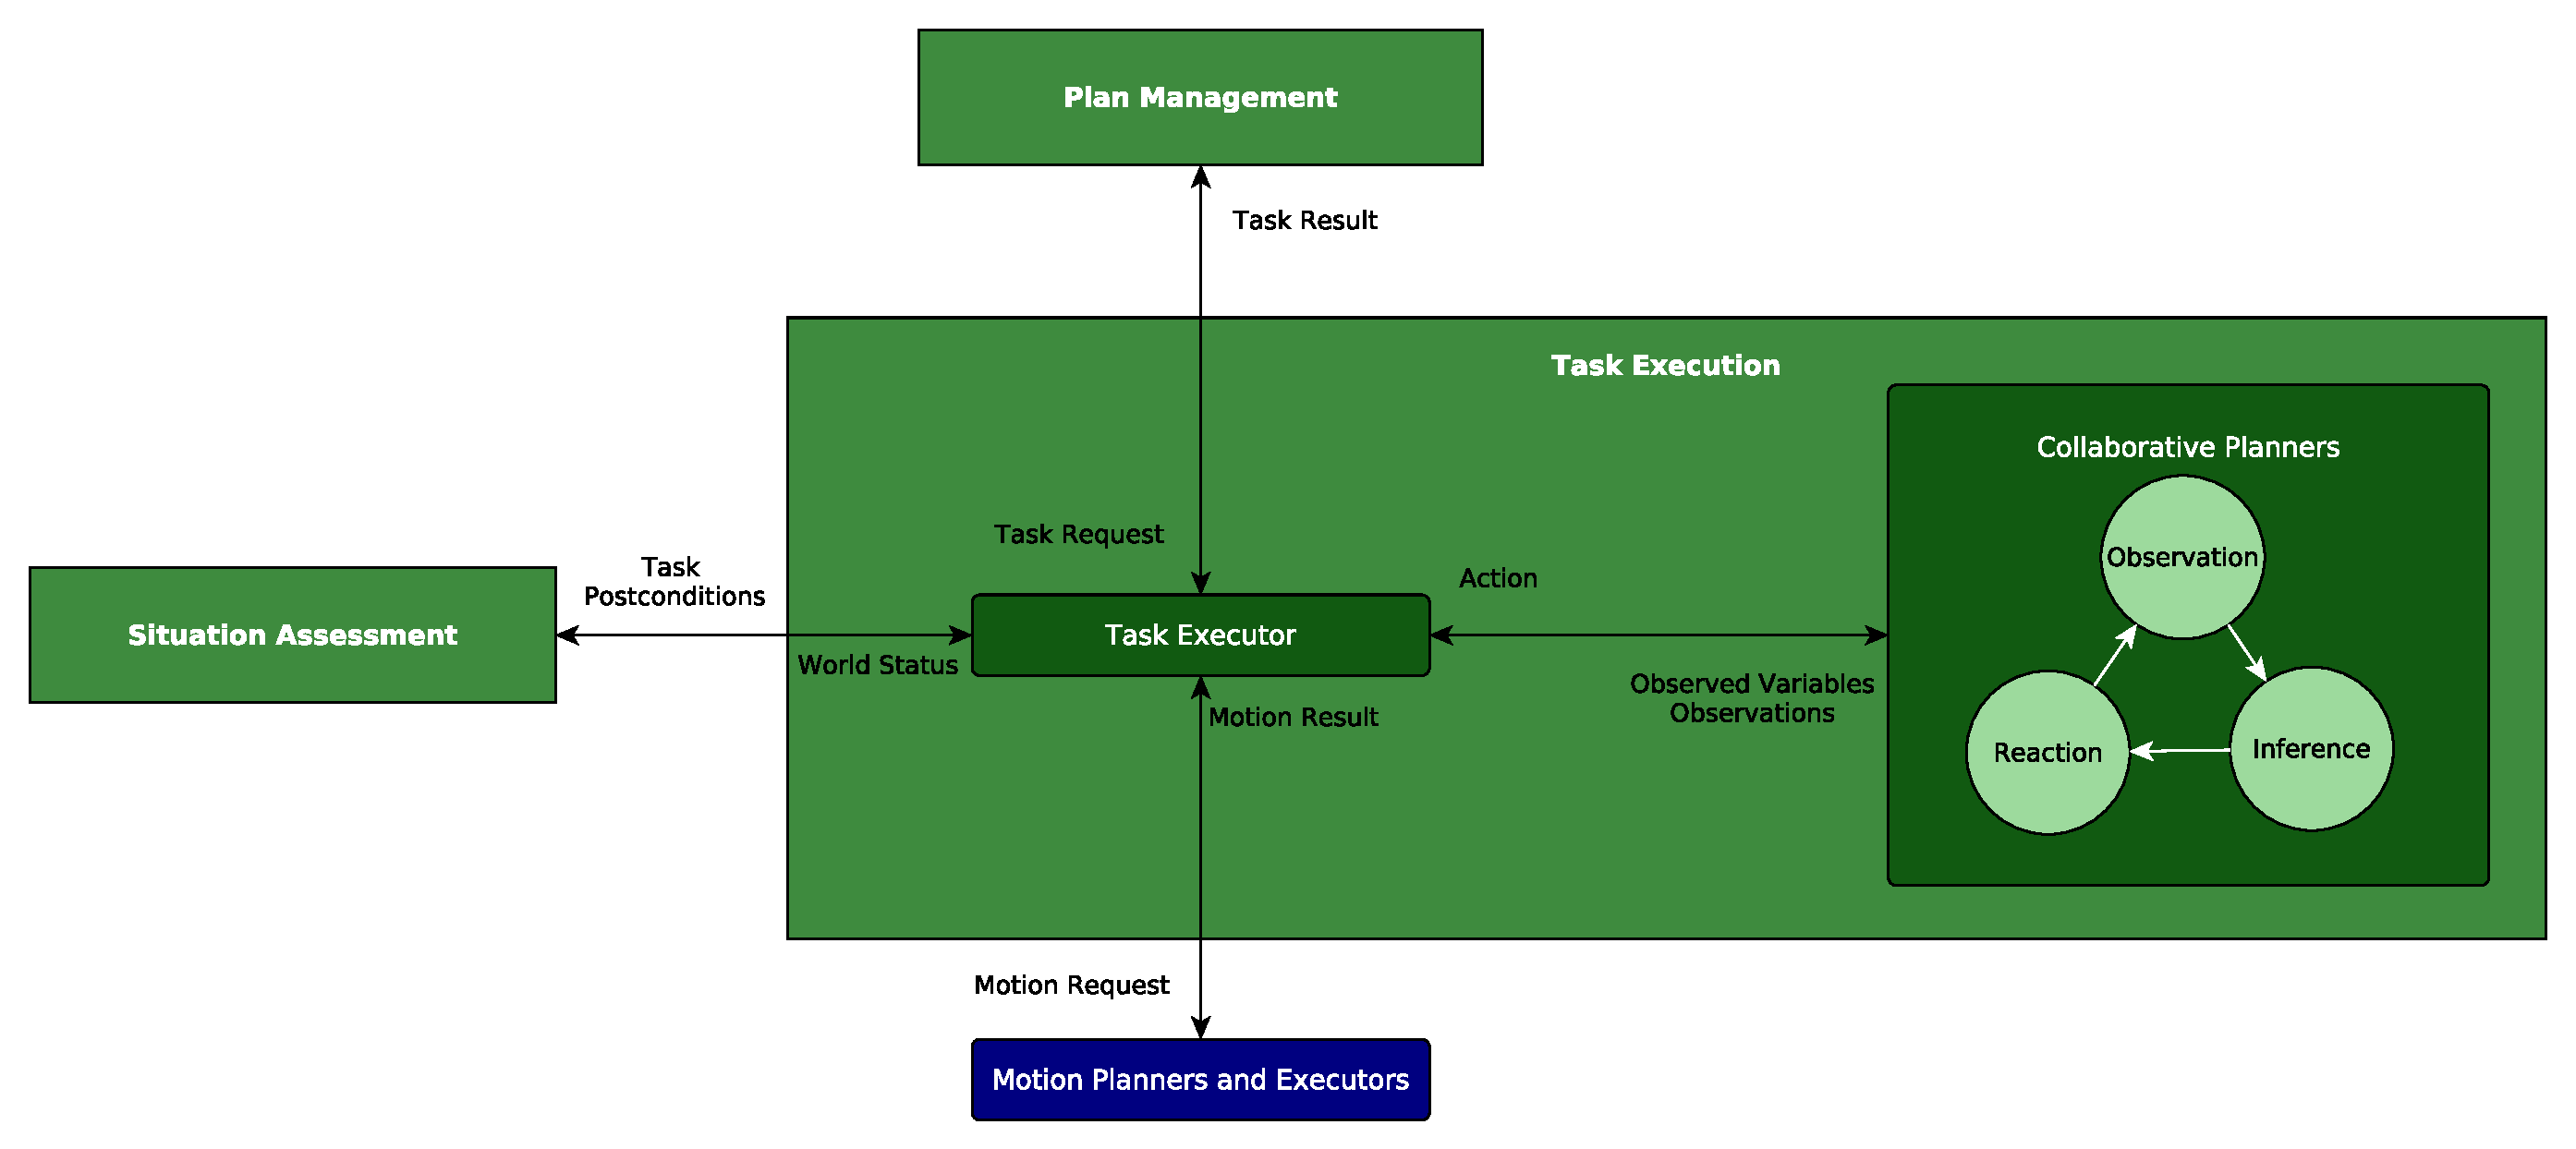
\includegraphics[clip,scale=0.38]{img/coworker/task_execution/architecture.pdf}
	\caption[The architecture of the Task Execution layer]{The architecture of the Task Execution  layer. Dark green rectangles represent modules, while light green rectangles layers. Blue rectangles represent external modules. Arrows represent messages exchanged between components, with the label detailing the message. The white ellipses, and their arrows, represent the process of the Collaborative Planners, explained in Section \ref{sec:task_execution-collaborative_planners}. While in this image we present the Collaborative Planners as a single unit, the system actually has a set of planners, and will choose, during the execution of a joint action, which one to use.}
	\label{fig:task_execution:architecture}
\end{figure}


Parts of this chapter where presented in~\cite{fioreiser2014}.

\section{Task Executor}
\label{sec:task_execution-action_executor}
The Task Executor handles task requests from the Plan Management layer. Following the ideas presented in section~\ref{sec:task_execution-overview}, the execution of a task is handled in several steps:
\begin{itemize}
\item Check Preconditions. The system can check if the preconditions of the task are valid by sending a query to the Situation Assessment layer. If the preconditions are not valid, the module returns an error.
\item Execute Task. The task is executed, by communicating with the Motion Planners and Executors and, if the current task is a joint action, with the Collaborative Planners.
\item Set Postconditions. The postconditions of the task are set in the Situation Assessment layer.
\end{itemize}

The execution of a task can fail, and in that case the world status is updated consequently. For example, if the robot is trying to pick an object, and the motion planner does not manage to compute a trajectory to reach it, the object will be considered as \textit{not reachable} by the robot in the current world status. When the Plan Management replans, the system could look for a plan where the robot changes position and tries again the pick, or even asks another agent to give him the object.

Tasks can be paused and resumed. We set a number of safety rules, where the robot will pause executing a motion if a human, or one of his body parts, is too close to the robot's grippers or arms.

The robot is also able to show some social clues during an action, for example by moving its head toward the tasks's $target$. 

\section{Collaborative Planners} 
\label{sec:task_execution-collaborative_planners}
When executing joint actions with humans, the robot needs to continuously observe its partner and react appropriately. The robot's action should be based on different aspects. First of all, the robot should act differently depending on the current status and level of advancement of the task. Second, the robot should consider the status of the world, in order to take appropriate actions. Then, as we said, the robot should observe its partner's behavior, which can give different information. Of course, the robot should coordinate with the human's movements. For example, if the two agents are performing an handover, and the human extends his hand, the robot should extend its arm to bring the object in a reachable position.

Observing the human's activities can give us more subtle information, that represent how much he is engaged in the task. For example, in the case of the handover, if the human is oriented toward the robot and extending his hand, we can assume that he is currently engaged and cooperating. If, instead, the human is looking in another direction, or moving away, we can infer that he is currently doing something else, and perhaps has even abandoned the task.

To reason on all these variables and produce an appropriate reaction, we introduced a special framework to manage cooperative actions, called the Collaborative Planners, based on hierarchical Mixed Observability Markov Decision Processes (MOMDP). A MOMDP can be modeled as a tuple $(S_h,S_o,A,T,R,\Omega,O,\gamma)$, where $S_h$ is the hidden state, $S_o$ is the observed state, $A$ is the set of actions, $T$ is the transition function, $R$ is the reward function, $\Omega$ is the observation function, $O$ is the set of observations, and $\gamma$ is a discount factor. More details about Markov Models are provided in appendix~\ref{appendix-methods}.

Using n MMODP we can model observed variables, like the task and world status, and hidden variables, like the engagement level of the human, which we can infer from observations. Using a hierarchy of models, as explained in \cite{pineau2001hierarchical}, we can represent complex scenarios and tasks with smaller, simpler models, that can be solved more easily, and expand them by adding more actions and complex behaviors as we see fit.

For each joint actions, we will introduce a new Collaborative Planner. When the system is executing a joint action between the robot and a human, the Task Executor will contact the related Collaborative Planner.  The Task Executor will send requests containing the observations and observed variables, used to update the MMODPs, and the planner will return a sub-action to execute. To maintain this model generic the Collaborative Planners will output high-level actions, which the Task Executor will adapt to the current situation. This process will continue until the joint action is achieved, the planner chooses to abandon the task, or there is a failure.

We provide a \textit{basic framework} that we use to implement Collaborative Planners, that can be adapted to the specific task. While it is not obligatory to implement a Collaborative Planner following these ideas, we believe that they offer a good basis for cooperative tasks:

\begin{itemize}
	\item $S_h=\{human\_commitment\}$
		\begin{itemize}
			\item $values(human\_commitment)=\{engaged,not\_engaged,not\_interested\}$.
		\end{itemize}  

		The human commitment to the task can be modeled as a hidden variable.  A user can be engaged in the task, meaning that he is actively participating; not engaged, meaning that he is currently not participating, but we expect that he will resume the task (imagine, for example, a user receiving a phone call while executing a joint task); or not interested, meaning that he has abandoned the task. 

		Modeling the human commitment is very important, since the robot should choose its action based on this variable, and of course on other task related variables. For example, if the user is not currently engaged in the task, the robot might choose to wait for him, or ask him if he has a problem. If he has abandoned the task, the robot might look for another plan, or ask the help of another human. If he is committed, the robot could proceed to accomplish the task, as long as the world state allows it.

	\item $S_o:\{task\_advancement\}$.
		\begin{itemize}
			\item $values(task\_advancement)=\{not\_started,started,completed\}$.
		\end{itemize}

		The status of advancement of the task can provide useful information to help the robot  choose its actions. A simple way to represent it is considering just an initial state, where the agents have decided to execute a cooperative task, but have not started executing it yet; a middle state, where the agents are working to complete the task; and a final state, where the task is completed. Different tasks could further refine this variable.
	\item $A:\{continue,wait,abandon,engage\}$.

		When building an action set, the developer should consider how much control the MOMDP should have over the robot's actions. In our implementations, we chose to plan generic high level actions, that will be adapted by the Task Executor. This strategy allows us to simplify the state space of the MOMDP. In a basic Collaborative Planner, the robot is able to: continue its task, meaning that it will take the next logical action depending on the current state, maintained by the Task Executor; wait for the user, if the robot detects that he is momentarily not engaged in the task; abandon, if the user is not interested anymore in executing the task; engage, to communicate with the user, for example by giving him a warning.

	\item $T$, $R$ and $O$ are, of course, completely dependent on the joint task.
	\item $\Omega$ is dependent on the current application. Some typical observations are related to spatial relationships between the user and the robot (e.g. the user is more likely to be interested in the task if he is close to the robot and oriented toward him), or particular poses of the user (e.g. the user is ready to receive an object if he has extended its arm toward the robot).

\end{itemize}

Our idea is similar to the work of \cite{ferrari2015hierarchical}. The authors propose a framework based on hierarchical POMDPs for cooperative tasks, with a three layer structure. This framework was applied to an escort application, where the robot had to guide a user to his location in a human-aware way, adapting to his behaviors. In this application, the commitment of the user is estimated by reasoning on how much the human is focused on the robot, and on their distance.
We implemented a similar application, for a robot guide, using our Collaborative Planners, which we will show in chapter~\ref{chapter:case_study}. The main difference between our framework and the one developed by the authors is that they chose to give a much stronger decision power to the POMDP, while in our system planning is actually split among several units, and the Task Execution module has a big role in adapting the actions of the Collaborative Planners. We also do note use a precise hierarchical framework, leaving to the single Collaborative Planners the choice on how many layers of task to use.

We will show, in the next section, an example of collaborative planner which develops this basic framework.

\section{Collaborative Planner for Handover}
\label{sec:task_execution-handover}
The handover collaborative planner has the goal to handle both human-robot and robot-human handovers in a human-aware way. We will show parts of this model now, avoiding the observation and transition function, as they are extensive and do not provide particular help in understanding this example.

\begin{itemize}
	\item $S_h:\{human\_commitment\}$.
		The hidden variable, and its values, follow the basic framework presented in the previous section.
	\item $S_o:\{task\_advancement\, timer, human\_distance\}$.
		\begin{itemize}
			\item $value(task\_advancement)=\{not\_started,started,touching,completed\}$.
			\item $values(timer)=\{not\_expired,expired\}$.
			\item $values(human\_distance)=\{close, far, out\_of\_range\}$.
		\end{itemize}

		The task advancement is represented in a similar way as the basic framework. We add the $touching$ value to this variable, representing the fact that the gripper of the robot has detected some pressure (e.g. the human has placed an object in it, if the handover is human-robot, or he has grabbed the object kept in the gripper, if the handover is robot-human).
		 We add a timer variable, which is started and controller by the Task Executor when the robot is waiting for the user. When the timer expires in the Task Executor, this variable will be set accordingly, and the robot can perform specific actions (e.g. ask the user if he still wants to perform the task).
		 We also consider the human distance from the robot, classyfing it as $close$ to the robot, $far$ from the robot, and $out\_of\_range$ if the human is not visible. 
	\item $A:\{continue,wait,abandon,engage\}$.

		The actions follow the basic framework. The $continue$ action is chosen when the user is $engaged$. The Task Executor will react differently to this action, dependingly on the current $task\_advancement$. If $task\_advancement \neq touching$ then the robot will extend (or keep extended) the arm toward the user. If $task\_advancement=touching$ the robot will release the object, or grab it from the human's hand, depending on the kind of handover.

		The $wait$ action is chosen when the user is $not\_engaged$. In this case the robot will retract its hand to an intermediate position. The Task Executor will start a timer.

		The $abandon$ action is chosen when the user is $not\_interested$ or the task is $completed$.

		Finally, the $engage$ action is chosen when the $timer$ is $expired$. In this case the robot will ask the human if he still wants to perform the handover.
	\item $O:\{human\_arm,human\_orientation,human\_distance\_variation\}$.
		\begin{itemize}
			\item $values(human\_arm)=\{approaching,retracting,still,unknown\}$.
			\item $values(human\_orientation)=\{toward\_robot,other,unknown\}$.
			\item $values(human\_distance\_variation)=\{decreasing,increasing,still,unknown\}$.
		\end{itemize}

		We present several human observations, used to estimate his engagement. In general, we consider that the human is more likely to be $engaged$ when he is approaching the robot, he is turned toward it, and his arm is extending. If the human is turned away, or even leaving, it is more likely that he is currently $not\_engaged$ or even $not\_interested$. Finally, if the human is $out\_of\_range$, his observations will be $unknown$, since the robot does not know his location.

	\item  $R$: the robot is rewarded for completing the task, performing the handover, and for executing desirable behaviors, like waiting for a user if we detect that he is not engaged, and abandoning the task if he is no longer interested in the joint action. 
\end{itemize}

An example of handover using this Collaborative Planner is shown in figure~\ref{fig:task_execution-handover}.

\begin{figure}[h!]
	\centering
	\includegraphics[scale=0.3]{img/coworker/task_execution/handover.pdf}
	\caption[Handover]{A robot-human handover}
	\label{fig:task_execution-handover}
\end{figure}
 
\chapter{Experiments and Results} % Main chapter title

\label{chapter:coworker_experiments} % Change X to a consecutive number; for referencing this chapter elsewhere, use \ref{ChapterX}

\lhead{Chapter 8. \emph{Experiments and Results}} % Change X to a consecutive number; this is for the header on each page - perhaps a shortened title

This chapter presents an experiment used to evaluate the robot coworker problem. Section~\ref{sec:coworker_experiments-scenario} introduces our scenario. Section~\ref{sec:coworker_experiments-experiment} shows our experiments. Finally, section~\ref{sec:coworker_experiments-discussion} presents and discusses our results.


\section{Scenario Description}
\label{sec:coworker_experiments-scenario}
In this section we show experiments created to validate our system in a domestic scenario, where the robot can help a human partner to achieve a joint task. This experiment was previously presented in \cite{fioreiser2014}.


We present a scenario where the robot, a PR2 by Willow Garage, and a human have a joint goal: cleaning a set of furniture. 
The environment is composed by two different furniture, a $TABLE$ and a $SHELF$, and three tapes,
 $TAPE1$, $TAPE2$ and $TAPE3$. The goal of the agents is throwing each tape in a $BIN$. We will present different examples, where the items will be placed differently, depending on our needs. The scenario is shown in figure \ref{fig:coworker_results-pr2helper}

 \begin{figure}[ht!]
 	\centering
 	\includegraphics[scale=0.45]{img/coworker/results/experiment.pdf}
 	\caption{The robot coworker scenario example, with a PR2 robot and a user.}
 	\label{fig:coworker_results-pr2helper}
 \end{figure}

In this scenario, human detection and handling was done using a depth camera, mounted on the ceiling. the scenario uses both the capacities of the robot coworker, described in this part, and the belief management and action inference capacities of the robot observer, shown in part~\ref{part:robot_observer}.

\section{Experiments}
\label{sec:coworker_experiments-experiment}
We will describe different experiments conducted in our laboratory.

\begin{itemize}
  \item
\textbf{Equal Partners}:
In this scenario (figure \ref{fig:coworker_results-scenario1}) the user is asked to clean the table, without explaining him what is the shared plan that will be used. The user is just informed that
the robot will try to help as it can to perform the task. The robot is already aware about the joint goal, but at the start of the scenario limits itself to monitor its partner.The user moves to the table and takes the \textit{TAPE2}. At this point, the robot infers that the user
has completed an action.
\begin{figure}
  \caption[Robot coworker experiment 1]{Robot adapts. This figure shows the robot's representation of the scenario. The white tape is the \textit{TAPE2}, while the blue
    one is the \textit{TAPE1}. The round shapes represent the agents'
    rechabilities, with red shapes representing robot reachabilities
    and green shapes human reachabilities. In this case only the human
  can reach the \textit{TAPE2} while both agents can reach the \textit{TAPE1}
and the \textit{BIN}. After the human takes the \textit{TAPE2} the
robot produces a plan where the human must throw the tape in the
bin while the robot can take the \textit{TAPE1} and throw it in the
bin.
}
\centering
  \subfigure{
  \includegraphics[scale=0.25]{img/coworker/results/scenario1.pdf}
  }
  \subfigure{
  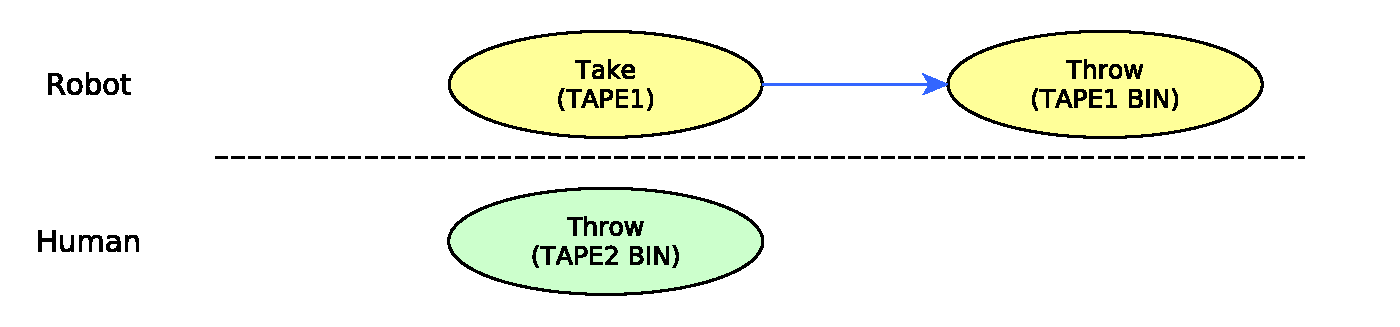
\includegraphics[scale=0.7]{img/coworker/results/plan1.pdf}
  }
  \label{fig:coworker_results-scenario1}
\end{figure}

The robot creates a plan and executes its part of it while monitoring the human,
who executes his part without deviating from the plan calculated by
the robot.

\item
\textbf{Modality switch and user plans}:
In this scenario (figure~\ref{fig:coworker_results_scenario2}) the robot is the only agent able to reach both tapes, but it can not reach
the bin, which can instead be reached by the human. We tested
this scenario in two different runs. In the first run, the current plan management modality is \textit{robot leader}.
After exploring the environment, the robot produces a plan and starts its execution.

\begin{figure}
  \centering
  \caption[Robot coworker experiment 2]{Modality switch and user plans. Another configuration of
    the environment, where the robot can reach the two tapes and the
    human can reach the bin. The robot generates an initial plan
  from this situation. The block surrounding the Give and Receive
  actions means that they are considered a single joint action.}
  \centering
  \subfigure {
    \includegraphics[scale=0.25]{img/coworker/results/scenario2.pdf}
   }
  \subfigure {
    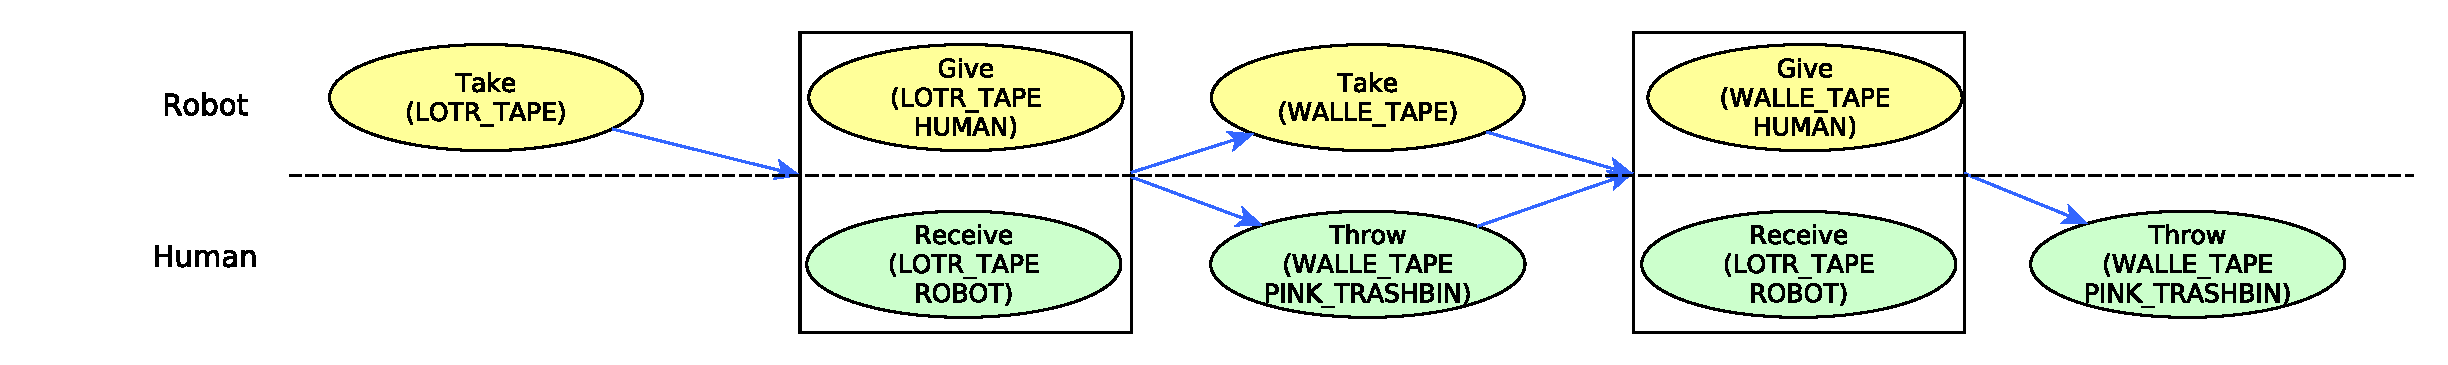
\includegraphics[scale=0.4]{img/coworker/results/plan2.pdf}
  }
  \label{fig:coworker_results_scenario2}
\end{figure}

While the robot is taking the \textit{TAPE1} the human moves
to take the \textit{TAPE2}. This deviates from the robot plan, so it
switches to the \textit{Equal Partners} modality, communicating the change to\
the user. The user throws the \textit{TAPE2} in the \textit{BIN} while
the robot takes the \textit{TAPE1} and handles it to the user. The user
takes the \textit{TAPE1} and throws it in the \textit{BIN}, completing the task.

In the second run the current modality is \textit{Human Leader} mode. The user is
asked to clean the table as he wishes. The user asks the robot to take
each tape and give it to him, throwing them in the trashbin.

\item
\textbf{Replanning after failed action}: 
In this scenario (figure~\ref{fig:coworker_results-scenario3}) the robot is the only agent able to reach the
bin, while both agents can reach the two tapes. The
robot is in \textit{Robot Leader} modality and, after examining the
environment, produces a plan.

\begin{figure}
  \caption[Robot coworker experiment 3]{Replanning after failed action. Here we can see a first
    plan, produced at the start of the scenario, and a second,
    produced after the robot fails to take the \textit{TAPE2}. }
  \centering
  \subfigure{
    \includegraphics[scale=0.25]{img/coworker/results/scenario3.pdf}
    }
    \subfigure {
      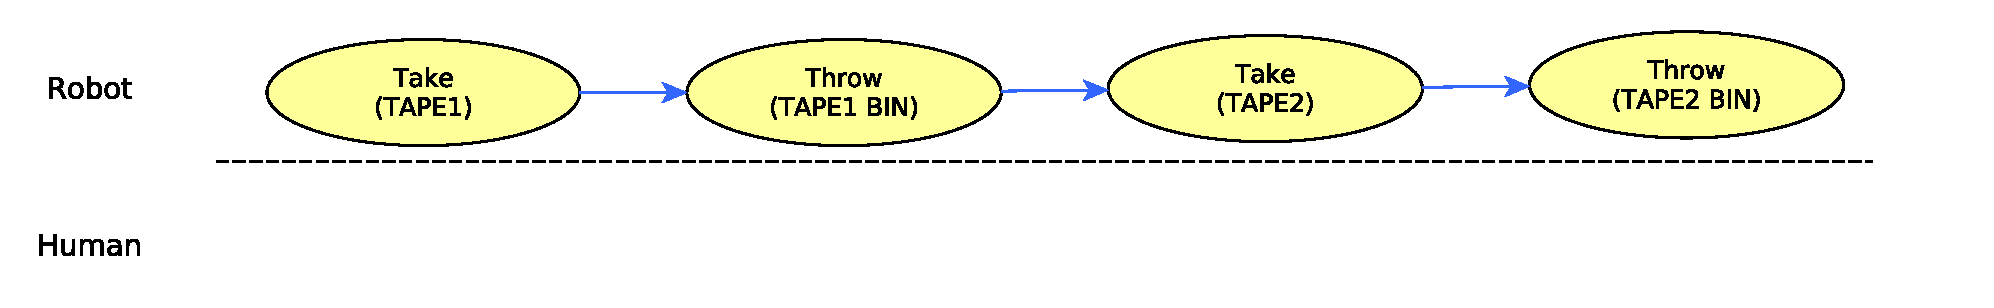
\includegraphics[scale=0.5]{img/coworker/results/plan3.pdf}

      }
      \subfigure {
        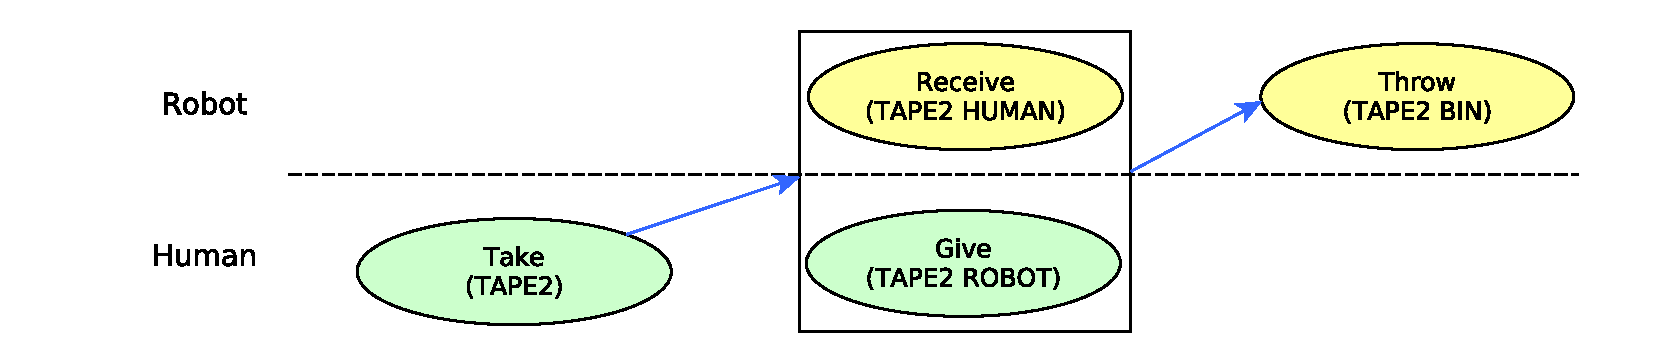
\includegraphics[scale=0.5]{img/coworker/results/plan4.pdf}
      }
  \label{fig:coworker_results-scenario3}
\end{figure}


After taking and throwing the \textit{TAPE1}, the robot tries to take the
\textit{TAPE2}, but fails because it is too far. The robot informs the user
and replans. The agents execute the plan, completing the task.

\item
\textbf{Replanning after human inactivity}.
In this run the robot computes that the \textit{TAPE3} and \textit{BIN}
are reachable only by the human, while the \textit{TAPE2} is reachable only by the robot. The robot computes a plan
and starts executing it, observing the human reactions. 
 After an initial stage when the human is
commited to the task, he does not execute a part of the plan (taking
the final tape and throwing it), so the robot looks for another
plan. The only solution to the problem is the one already computed at
the beginning, so the robot decides to ask
 the human to take the tape and throw it. A run of this
scenario is shown in figure ~\ref{fig:coworker_results-experiment}. 
\end{itemize}

 
\begin{figure}
  \caption[Robot coworker experiment 4]{The picture shows a run of our \textit{replanning after human
    inactivity scenario}. The different
    rows show, starting from top to bottom: the real world picture,
    the world state representation built by the robot, symbolic facts
    introduced in the knowledge base at each time step, action taken by the
    agents at each time step, the current plan calculated by the robot.}
  \centering
  \includegraphics[angle=90, scale=0.7]{img/coworker/results/complete_plan.pdf}
  \label{fig:coworker_results-experiment}

\end {figure}


\section{Discussion}
\label{sec:coworker_experiments-discussion}
We review some of the main results of our experiments in this scenario:
\begin{itemize}

\item
\textbf{The system is able to handle joint goals}.
The system is able to create shared plans with different users, taking
into account the capabilities of each agent. When unexpected changes
in the world or task status arise, the system is able to quickly
replan, adapting to new scenarios. The system is able to execute this
joint goal in a human aware way. 
                                
\item
\textbf{The system is able to handle joint actions}.
The system is able to estimate user intentions in collaborative tasks and to choose appropriate actions, using a set of MOMDP models.

\item
\textbf{The system is able to handle user preferences}.
The system is able to adapt itself to user preferences, allowing the
human partner to give commands or to be more passive in its role and
switching from one modality to the other. 
\item
\textbf{The system is able to handle each agent beliefs}.
The system is able to represent different belief states for different agents and to take into accout what users can see, reach and know when creating a plan.

\item
\textbf{The system is able to monitor human actions}.
The system was able to understand when the human performed action such as taking or throwing objects.
\end{itemize}

 
\chapter{Human-Aware Probabilistic Planning}
\label{chapter:mamdp}

\lhead{Chapter 9. \emph{Human-Aware Probabilistic Planning}} % Change X to a consecutive number; this is for the header on each page - perhaps a shortened title

In this section we present a recent work where we developed a Multi-Agent Markov Decision Process (MAMDP). Section~\ref{sec:mamdp-intro} presents the problem. Section~\ref{sec:mamdp-overview} briefly introduces our approach, which is explained fully in section~\ref{sec:mamdp-single_agent} and section~\ref{sec:mamdp-mamdp}. Section~\ref{sec:mamdp-discussion} discusses the characteristics of this model, while section~\ref{sec:mamdp-example} show an example of creation of a MAMDP, starting from single-agent models. Finally, section~\ref{sec:mamdp-plan_monitoring} proposes an extension to the plan monitoring algorithm previously introduced, that would allow our system to monitor tasks and evaluate human engagement in collaborative activities.


\section{Introduction}
\label{sec:mamdp-intro}
Multi-Agent planning   is an important and studied topic in the AI community \citep{durfee1999survey}. There are several approaches to this problem, using classical or probabilistc planning. There are several issues to consider:
\begin{itemize}
\item Distributed vs Centralized. A multi-agent planner might be distributed, meaning that separate systems plan independently and then communicate to build a shared plan (an idea investigated, for example in \cite{nikolaidis2013cross,guestrin2002distributed} ); or centralized, meaning that a single system plans for all the agents.
\item Coordination. Agents need to coordinate their plans, in particular in the presence of shared resources. Imagine, for example, two agents, Max and Bob, that are using a tool to repair a set of cars. If Max is proceeding faster than Bob and the two do not coordinate, Max might take the tool and leave, starting to repair another car, ignoring the fact that Bob still needs the tool. This example shows that it is important to reason on the duration of actions performed by agents. At the simplest level, agents need to know the advancement of the sub-plan of other agents. More complex reasoning might take into account how long an agent needs to perform a certain sub-task, in order to refine a plan. 
\item Cooperation. Even when performing different sub-tasks of the same plan, agents can help each other, for example by passing items, thus improving the efficiency of the plan. Multi-Agent problems can be loosely or tightly coupled, depending on the quantity of interactions between agents. Some works are not focused specifically on tightly or loosely coupled problems, and try to present a generic approach. \cite{torreno2015approach} proposes a cooperative refinement planning approach, based on the partial-order planning paradigm. In this work each agent refines a centralized plan. Agents are able to exchange information, since the complete world-state might not be observable by everyone. Refined plans are then analyzed by each agent, and voted with a democratic leadership approach. Results show that this approach is very efficient at solving loosely coupled problems, but also competent on tightly coupled situations. 

\item Communication and Knowledge. In a multi-agent environment each agent might have an incomplete or incorrect belief on the world, which might lead to wrong or sub-optimal actions. Agents may communicate to progressively build a correct belief model on the world state. 
\end{itemize}

Several approaches has been studied to bring the multi-agent planning problem in a probabilistic framework. \cite{boutilier1999sequential} create a centralized MDP, able to select at each time step actions for every present agent. Dec-POMDP \citep{bernstein2002complexity} and I-POMDP \citep{gmytrasiewicz2005framework} are more complex frameworks, that take into account the belief models of agents. The complexity of these models makes them difficult to use in even moderately difficult scenarios. A solution to this problem is considering simpler problems, where the agents mostly work independently and interact only in limited situations, such as in \cite{melo2013heuristic}.  Since we are more interested in tightly coupled scenarios, where the robot and human interact often, these kind of approaches are not suitable.

\section{Overview}
\label{sec:mamdp-overview}
In some situations, the environment, or other agents' actions, can be very unpredictable, and the system needs to constantly adapt its plans to the current state of the world, by replanning or repairing processes, which can be expensive. To deal with this issue we developed a Human-Aware Probabilistic Planner, based on MDPs. Our goal is replicating the characteristics of HATP, which we presented in section~\ref{sec:plan_management-hatp}, in a probabilistic domain. We designed this planner with the following ideas:

\begin{itemize}
\item Centralization. We will use a single planner, which chooses actions for all the involved agents.
\item Hierarchical. The domain will be split in different modules, which interact to achieve the goal. Hierarchical models allow us to speed up the computation of the MDP policy and to reuse models in different domains and tasks.
\item Tightly Coupled. We will focus on problems where the agents' interactions are frequent.
\item No Communication. The planner will  assume that all the agents have perfect knowledge of the world state. The rest of the system will have to take care of maintaining users' knowledge, ensuring the correct execution of the plan. Current planners that try to include communication issues often focus on loosely coupled interactions between the agents, in order to simplify the domain and be able to compute a policy for the problem. Since we choose to focus on tightly coupled problems, we can not use this solution, and so prefer to avoid the issue at this level.
\end{itemize}

This work is a very recent development, and has not yet been integrated in the rest of the system. We will explain the main characteristics of the MAMDP in the following sections.


\section{Single-Agent MDP}
\label{sec:mamdp-single_agent}
The starting point for this planner is the single agent MDP. We start with the classical model \\ $(S,A,T,C,G,S_0)$, where $S$ is the system space, $A$ is the set of actions, $T(s_i,a,s_j)$ is the probability to transition from state $s_i$ to state $s_j$ after taking action $a$, $C(s,a)$ is the cost of taking action $a$ in state $s$, $G \in S$ is the set of goal states, and $S_0 \in S$ is the set of starting states. We express the state space $S$ of the system as a set of variables $var$, each one with a possible range of values $values(v)$, where $v$ is a variable.

 We develop this model in the following way.

\subsection{Parameters}
We can define parameters in our MDP, and assign them to different values. We will call the list of parameters of a MDP $par$ and their current instantiation the \textit{parameter\_instance} of the model. Parameters can be linked to variables and values. We call $par\_var$ the variables associated to a parameter. 

For example, let us imagine a scenario of a room, with different furniture and objects. Let us define the state space of a generic MDP to take an object in this room. We can define two variables: the location of an agent, \textit{agent\_isAt}, which can assume values in the set ${f_1, f_2, f_3}$ (where $f_i$ represent a furniture in the room); and an object variable, \textit{object\_isAt}, which can assume the same values as the \textit{agent\_isAt} variable. If we define two parameters, \textit{agent} and \textit{object}, and link them to the \textit{agent\_isAt} and \textit{object\_isAt} variables, we can create a generic MDP which can be used to plan for any agent (with similar capacities) to take an object in this room.

The MDP receives as input, when consulted to select an action, the state of the world,  which we will call \textit{real\_space}. The \textit{real\_space} will be converted, using the \textit{parameter\_instance}, to the \textit{parameter\_space}, which will be actually used by the model in its computations. 

For example, in the real world, we have two agents, \textit{Bob} and \textit{Greg}, and three objects \textit{glue}, \textit{book}, \textit{smartphone}. If we assign the \textit{agent} parameter to \textit{Bob} and the \textit{object} parameter to \textit{book}, when receiving the complete world state the MDP will assign as \textit{agent\_isAt} the location of Bob, and as \textit{object\_isAt} the location of the book, discarding unneeded variables.

Parameters allow us to create smaller, generic MDPs, which can be reused easily.


\subsection{Actions and Macro Actions}
We define actions as a tuple $(subject,action\_name,object,target)$, where each element of the tuple is called an $action\_part$.  We represent the action as a string, composed by its $action\_parts$, joined by the character `\_' as delimiter. For example, an action where Greg places a book on a table can be represented as \textit{Greg\_place\_book\_table}. We define the function $convertPar(a)$ and $convertReal(a)$ to convert action $a$ to the \textit{real\_space} or the \textit{parametrized\_space}.

We add to the normal set of actions of a MDP \textit{macro actions}, linked to other MDPs, which allow us to create a hierarchy of MDPs. We call $M$ the set of \textit{macro actions} of the MDP, and $sub(a)$ the sub-MDP linked to the \textit{macro action} $a$. For example, we might create, in a MDP whose goal is cleaning a room, a macro action to reorder the room's objects and one to clean the floor. Each of these macro actions will be linked to a specific MDP, who will refine the problem in more details.

The cost of executing a macro is directly computed from the sub-MDP. There are several strategies to compute this cost, like in \cite{dietterich2000hierarchical,hauskrecht1998hierarchical}.

\subsection{Name and Parameter Name}
We define for each MDP model a \textit{name}, which identifies it, and a \textit{parametrized\_name}, which substitutes parameters using the \textit{parameter\_instance}. The \textit{name} is defined using the same tuple as an action. 

For example, a MDP whose goal is to obtain an object could have as \textit{name} $agent\_get\_object$ and as \textit{parametrized\_name}, in a certain moment, $Greg\_get\_book$.

We define a function $assignParameterFromActionName(a)$ which creates the \textit{parameter\_instance} of the MDP based on an action name. This function can be very useful when using \textit{macro actions}, so that the system can assign parameters to the sub-MDP from the \textit{macro action} string and then consult it.

For example, if the \textit{macro action} $Greg\_get\_book$ is linked to the $agent\_get\_object$ MDP, this function would assign values to the  $agent\_get\_object$ model's parameter. The system would assign the value $Greg$ to the $agent$ parameter and the value $book$ to the $object$ parameter. 

Each \textit{name} can be divided in a number of $name\_parts$,  with the same procedure as actions. The \textit{parametrized\_name} can be divided as well in $parametrized\_parts$.


\subsection{Abstract States}

In some situations, a model might not need to base its planning choices on all the possible values of a variable in the \textit{real\_space}. Imagine, for example, the case where an agent needs to perform a series of operations on the furniture $f_1$ in the room. In this case, we could model the  values of the \textit{agent\_isAt} variable as $\{f_1 , other\_location\}$, greatly reducing the state space. In this situation we say that \textit{agent\_isAt} is an \textit{abstract variable}. 

We build a map $abstract\_values_v$ for each abstract variable $v$, which links real world values to model values (e.g. $f_2 \rightarrow other\_location$). This map will be used to convert a state expressed in the $real\_space$ to the $parameter\_space$ of the model. 
%The choice of using abstract variables needs to be carefully weighted, because they can impact on the quality of the solution of the model.

\section{Multi-Agent MDP}
\label{sec:mamdp-mamdp}
Now we will explain how we build a Multi-Agent MDP (MAMDP), starting from $n$ single-agent models, one for each agent. We will call the single-agent models $MDP_i$, where $1 \leq i \leq n $ is the index of the agent. In the following paragraphs, we will use the notion $S_i, var_i, values_i, A_i, T_i, C_i, G_i, S_{0i}, M_i, par_i, par\_var_i$ when referring to components of the single-agent MDP, adding the $i$ index to differentiate them from the MAMDP. 
 
\subsection{Name and Parameter Name}
The \textit{name} and \textit{parameter\_name} of the MAMDP are built by concatenating those of its agent MDPs, adding the `-' character to separate the single agents.

For example, the \textit{name} of a MAMDP with single-agent models \textit{agent\_get\_object} and  \textit{agent\_clean\_table} is \textit{agent\_get\_object-agent\_clean\_table}.

\subsection{State Space and Parameters}
$par=\bigcup_{1 \leq i \leq n, p \in par_i} p+\text{`p'}+i $ \\
$par\_var=\bigcup_{1 \leq i \leq n, v \in par\_var_i} \> rename(v)$ \\
$var=\bigcup_{i=1}^{n}(var_i \setminus par\_var_i) \cup par\_var$ \\
$\forall_{v \in var}\> values(v)=\bigcup_{i| v \in var_i} 
\begin{cases}
	 values_i(v) \quad \text{if } v \not \in par_i \\
	 p+\text{`p'}+i \quad \text{if } v \in par_i \\
\end{cases}$ \\ 

To create the set of parameters of the MAMDP we will rename each parameter in the single-agent MDPs, adding an identifier composed by `p' and by the index of the MDP. We make this choice because different MDPs could share the same parameters, but they could be assigned to different values, and so need to be treated as separate entities, even if they have the same semantic meaning. Parameter variables are created by renaming the parameter variables of the sub-MDPs to account for this newly added identifier.

For example, if the $MDP_1$ model has a parameter \textit{object}, linked to a variable called \textit{object\_isAt}, we will rename the parameter as \textit{objectp1} and the variable as \textit{objectp1\_isAt}. 

We defined $S$ as the union of the variables of the single-agent MDPs excluding their parameter variables. We will instead take the parameter variables of the MAMDP, in the way that we just defined.

The MAMDP variable can assume all the possible values that are available in the corresponding variables of the sub-MDPs. As before, we will change values that are parameters to account for our renaming procedure. 

We define the function $single_i(s)$ , which converts the MAMDP state to state of the single-agent MDP $i$.


\subsection{Actions}
$A=(\prod_{i=1}^{n} A_i) \cup JointActions \cup WaitActions$ , where $JointActions$ is the set of collaborative actions, and $WaitActions$ is a set computed by enumerating all the possibile instances where one or more agents do not act, and simply wait, while others are acting.

The actions of the MAMDP are a concatenation of the actions of the single MDP, adding the separator character `-' between the different agents' actions. We will refer to the single agent's actions of action $a$ as $a_i \quad \forall \> 1\leq i \leq n$.

For example, the MAMDP will contain actions such as `agentp1\_move\_surface1-agentp2\_move\_surface2'.

We add to $A$ the special set of $JointActions$, which are actions that the agents can use to cooperate. For example, if there is a resource in a single agent MDP which two agents can possess, we introduce a $handover$ action between them. 

For each $a \in A$, if there is a sub-action $a_i$ which is a macro action for MDP $i$, we create a new MAMDP and assign it as sub-MAMDP of $a$. This sub-MAMDP will be created from $n$ MDP models, as for its father, in the following way. Let $f$ be the father MAMDP, $c$ the sub-MAMDP, and $a$ the macro-action of $f$. \\
 $ \forall_{\text{MDP}\> m_i \in f}$ we assign a MDP $m_j$ in $c$ where:\\
$m_j= \begin{cases}
	m_i & \quad \text{if } a_i \not\in M_i \\
	sub_i(a_i) & \quad \text{if } a_i \in M_i 
\end{cases}$ \\

\subsection{Transition Function}
\label{subsec:mamdp-transition}
$T(s_a,a,s_b)=
\begin{cases}
\prod_{i=1}^{n}(T_i(single_i(s_a),a_i,single_i(s_b))) & \> \text{if } !isIncongruent(s_a)\; \land  \;!isIncongruent(s_b)  \\
0   & \quad \text{else}
	\end{cases}$ \\

The transition function is computed as the product of the transition functions of the single agent MDPs, on the converted states and actions.

We set the probability as zero if either the starting or ending states state of the transition are incongruent. This is done by converting the states to the \textit{real\_space} and checking the values of the different variables. We say that a state is incongruent if two non abstract variables in the \textit{parameter\_space}, that are assigned to the same \textit{real\_space} variable, have different values. If one or both the variables are abstract we check if their $abstract\_values$, for the current variable values, have a value in common. If not, we consider the state incongruent.

For example, consider the state $(objectp1\_isAt=`surface', objectp2\_isAt=`table', agentp1\_isAt=`table', agentp2\_isAt=`table')$. If in the current \textit{parameter\_instance} both \textit{objectp1} and \textit{objectp2} are assigned to the same variable, this state will be incongruent.

Consider now the state $(objectp1\_isAt=`agentp1', objectp2\_isAt=`other', agentp1\_isAt=`table', \\ agentp2\_isAt=`table')$. If $objectp1$ is a parameter assigned to $Greg$, \textit{objectp1\_isAt} is an abstract variable, and $abstract\_values_{objectp2\_isAt}(`Greg')=`other'$, this state will not be considered incongruent.  


\subsection{Start and Goal States}
$S_0=s \in S\; | \; \forall_{i=1}^n s_i \in S_{0i} $. A state is a starting state in the MAMDP only if it is a starting state in all the single agent MDPs.\\
$G=s \in S\; | \; \exists_{i=1}^n \; | \; s_i \in G_{i}$. A state is a goal state in the MAMDP if it is a goal state in any one of the single agent goal states. The idea of this choice is that a MAMDP terminates when one of the agents has achieved its goal. If there is an agent that has not completed its task, and the MAMDP was a sub-model in a hierarchy, its father will select another action, perhaps assigning one or more agents to the incompleted task. 

In some situations, we might try creating a MAMDP composed of opposing goals, like for example, a MAMDP where both agents need to get the same object. Since we are interested in cooperative and not competitive scenarios, we will not create these kind MAMDPs. We can recognize this situation by checking if there is any state in $G$ that is incongruent, as previously defined in subsection~\ref{subsec:mamdp-transition}. 


\subsection{Cost Function}
$C(s_a,a,s_b)= 
	\begin{cases}
		max_{i=1}^{n}(C_i(single_i(s_a),a_i,single_i(s_b))  & \quad \text{if } s_b \not\in G \\
		\sum_{i | single_i(s_a) \not\in G_i} expectedCost_i(single_i(s_a))  & \quad \text{if } s_b \in  G
		\\
	\end{cases} $	\\

where $expectedCost_i(s)$ is a function that computes the expected cost for agent $i$ to reach a goal state by starting in state $s$ and following the action policy. In this calculation, we allow from the other agent only $JointActions$ that are necessary to solve the plan (e.g. handovers if the agent does not have a needed resource).

The cost function of the MAMDP is chosen by taking the maximum cost of the single agent actions that are executed, if the state $s_b$ is not a goal state. If it is a goal state, we take as cost an estimation of the time required by any agent that has not reached his goal to complete their tasks, with only minimal cooperation. In this way, we encourage the MAMDP to choose plans where the agents cooperate and do not only try to achieve their goal.

\section{Discussion}
\label{sec:mamdp-discussion}

The result of this fusion is a MDP, that can be solved with well-known algorithms, like value iteration. By fusing all the possible MDPs, the resulting model can be  very hard to solve but, using macro actions, parameters, and abstract states we can greatly reduce its complexity. 

The action space of the joint model is calculated as the cross product of the action spaces of the single model. When there are several macro actions in the agent models, this could result in the creation and computation of the policy of several sub-models, which can significantly slow down the computation of a solution for the model. We can reduce the complexity of this process by making several considerations.

First of all, created MAMDPs can be reused in different branches of the hierarchy, if needed. When creating a new MAMDP, we will look to see if there is already an existing MAMDP with the same $name$ and, if so, we will use it.

Second, parameters can greatly  reduce the number of sub-MAMDPs to compute. Let $a$ be a \textit{macro action}, $c$ the sub-MAMDP linked to $a$, $1..n$ the indexs of the single-agent MDPs of $c$, which are selected as previously explained.

 We create the \textit{parametrized\_name} of $c$ by concatenating the \textit{parametrized\_name} of its single-agent MDPs. To set the $name$ of  $c$ we process each name of its single-agent MDPs $name_i$, by modifying all of its $name\_parts_{i,k}$, with $1 \leq k \leq m$ in the following way:\\
$name\_part_{i,k}=
\begin{cases}
	name\_part_{i,k} & \quad \text{if } !parametersInCommon(name\_part_{i,k}) \\
	parametrized\_part_{i,k} & \quad \text{else}
\end{cases}$ \\
where $parametersInCommon(name\_part_{i,k})$ is a function that returns true if $name\_part_{i,k}$ is a parameter in sub-MDP $i$, and there is a sub-MDP with index $j$, where $name\_part_{i,k}$ is a parameter or variable. \\

The idea behind this choice is the following. If the sub-MDPs do not have parameters in common, we can use a generic MAMDP to represent this instance. For example, if we create a MAMDP for the macro action $agent1\_clean\_table-agent2\_clean\_shelf$, we can use the MAMDP $agent\_clean\_furniture-agent\_clean\_furniture$ since the sub-MDP models do not have parameters in common, and their actions will not conflict.

 If instead we create a MAMDP for the macro action $agent1\_clean\_table-agent2\_clean\_table$ we create a specialized MAMDP, since there are parameters in common ($table$) and if we treat them as different objects there could be incongruences in the MAMDP planning.



\section{Example}
\label{sec:mamdp-example}
In this section we will show an example of creation of a MAMDP. We start by presenting a cooperative scenario. The robot and a human are working together to assemble three brackets on three differents work surfaces. To assemble a bracket the agents need to clean the surface, apply some glue to it, and fix the bracket. A possible set-up for this scenario is shown in figure ~\ref{fig:mamdp-mamdp_scenario}.

 \begin{figure}[ht!]
	\centering
	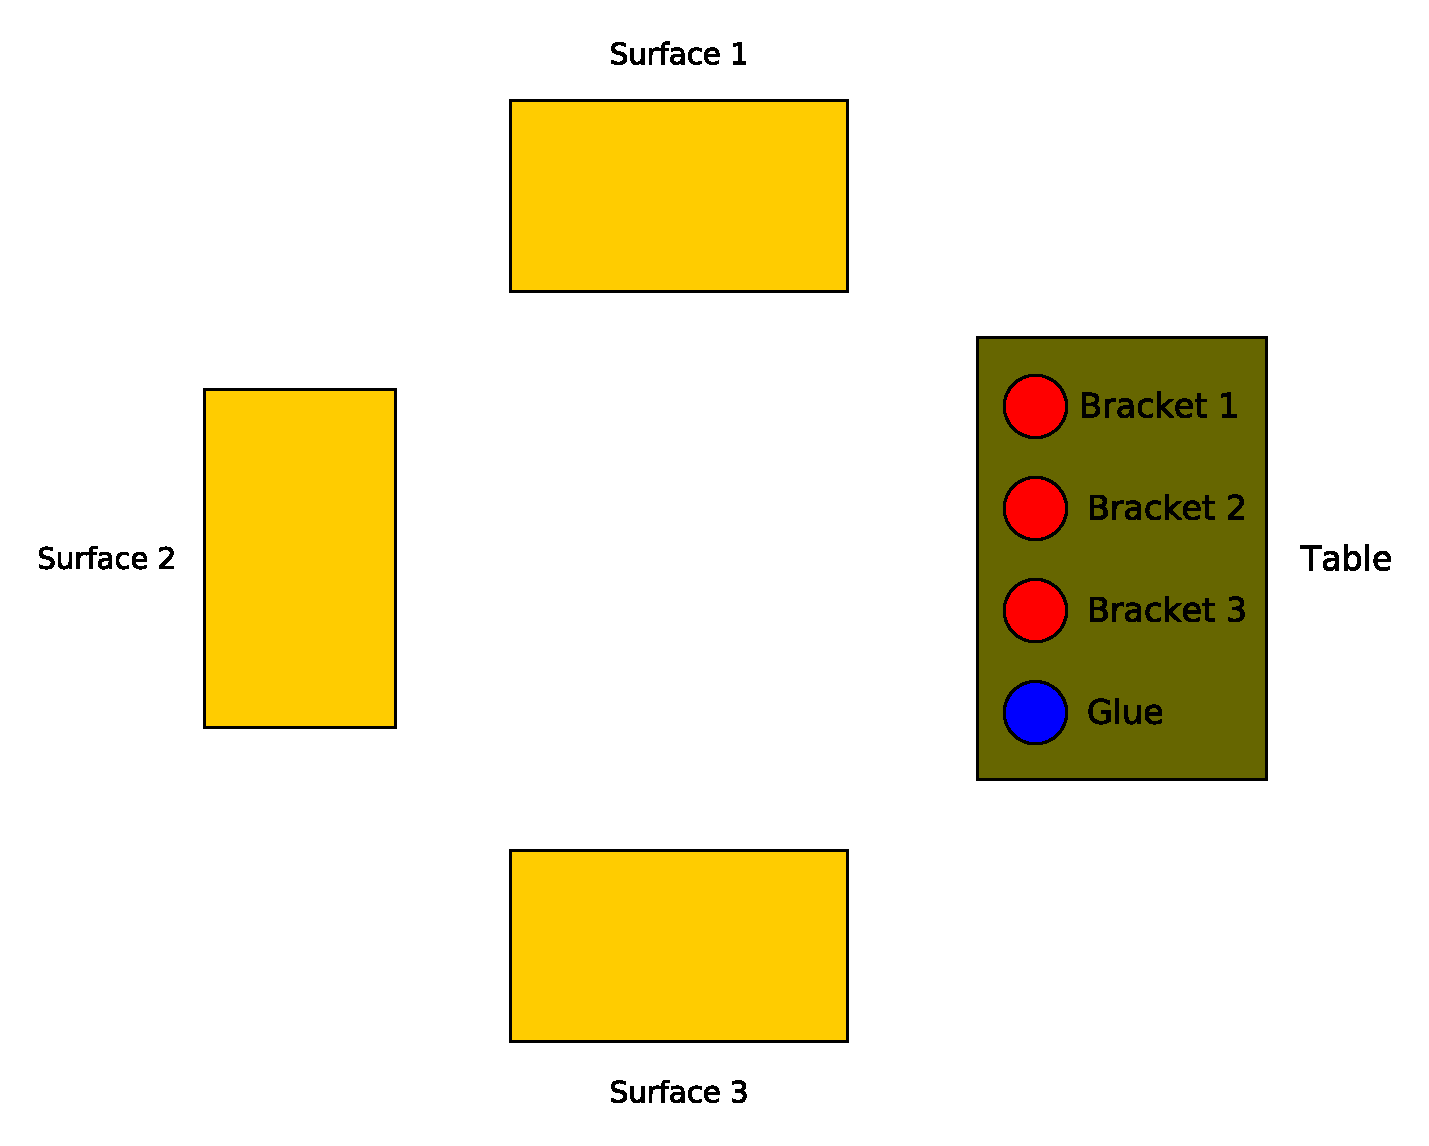
\includegraphics[scale=0.5]{img/coworker/mamdp/scenario.pdf}
	\caption[MAMDP example: scenario]{The image shows the set-up for this example scenario. The four locations are represented as different rectangles and the objects as circles. }
	\label{fig:mamdp-mamdp_scenario}
\end{figure}

\subsection{Single-Agent MDP}

We start by defining a single-agent MDP for this scenario. We will use a hierarchical architecture, as shown in figure~\ref{fig:mamdp-scenario_single_architecture}. This architecture is composed by three different modules: AssembleAllBrackets, which controls the flow of the scenario; AssembleBracketSurface, which assembles a chosen bracket on a chosen surface; and GetObject, which obtains an object. We will create some simplifications in these models, as they are chosen just to explain how we build a MAMDP, and not for a realistic use.

\begin{figure}[ht!]
	\centering
	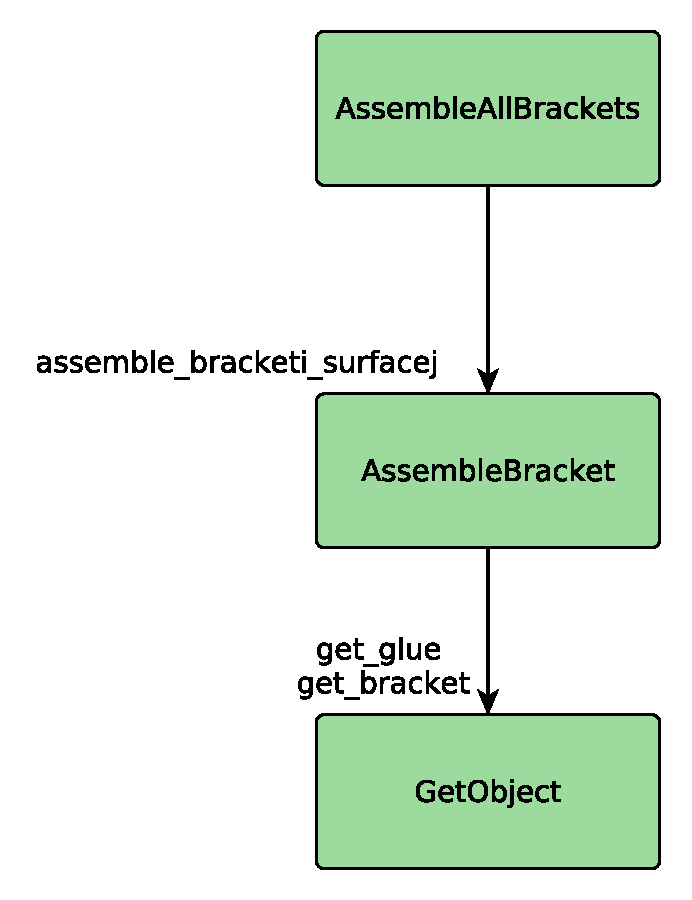
\includegraphics[scale=0.5]{img/coworker/mamdp/scenario_single_architecture.pdf}
	\caption[MAMDP example: single MDP model]{The image shows the architecture for the single agent MDP of the MAMDP example scenario. The various MDPs are represented as rectangles. The arrows show the links between hierarchical modules in the architecture. The label of the arrow shows the macro action corresponding to the link. The label \textit{assemble\_bracketi\_surfacej} actually correspond to all the combinations to assemble a bracket on a surface. We grouped them since, as the AssembleBracketSurface MDP uses parameters, it can be used for all these macros.}
	\label{fig:mamdp-scenario_single_architecture}
\end{figure}



\subsubsection{AssembleAllBrackets}
We will now show the \textit{AssembleAllBrackets} model, whose goal is directing the flow of the scenario, by choosing which bracket should be assembled on which surface.

\begin{itemize}
	\item $name: agent\_assembleallbrackets$.
	\item		$par: agent$.
		\begin{itemize}
			\item $par\_var(agent)=agent\_isAt$.
		\end{itemize}
		In this example, we decided to create generic models which can plan either for Greg or for the robot.
	\item $S:\;\{agent\_isAt,bracket1\_isAt,bracket2\_isAt,bracket3\_isAt,surface1\_status,\\ surface2\_status,surface3\_status\}$. 
		\begin{itemize}
			\item $values(agent\_isAt):\{table,surface1,surface2,surface3\}$.
			\item $values(bracketi\_isAt):\{table,surface1,surface2,surface3,agent,other\_agent\} \forall_{i=1}^3$. 
			\item $values(surfacei\_status):\{completed,other\_status\}\;\forall_{i=1}^3$.
		\end{itemize}
		\begin{itemize}
			\item $abstract\_values\_surfacei\_status:$ 
				\begin{itemize}
					\item $none: other\_status$.
					\item $cleaned: other\_status$.
					\item $glued: other\_status$.
				\end{itemize}
			\item $abstract\_values\_bracketi\_isAt$ 
				\begin{itemize}
					\item $greg: other\_agent$.
					\item $robot: other\_agent$.
				\end{itemize}	
		\end{itemize}
		The state set of the model contains the location of the agent, of the brackets, and the status of the surfaces. The agent and the objects can be located at the table or at one of the surfaces. In addition, objects can be possessed by another agent. The status of a surface can be set to none, meaning that the fixing process as not started; cleaned, meaning that the agent has already cleaned the surface; glued, meaning that the agent has applied glue to the surface; and completed, meaning the a bracket ha been fixed on it. 

		To simplify the model we consider the states $none,cleaned,glued$ as abstract states. We also consider $other\_agent$ as an abstract value, assigned to both agents present in the scenario. Let us consider, for example, that the instance of the \textit{agent} parameter is \textit{greg}, and that in the \textit{real\_space} \textit{bracket1\_isAt=greg}. It could seem that, when converting from \textit{real\_space} to \textit{parameter\_space}, the system would assign \textit{bracket1\_isAt} to \textit{other\_agent}, since \textit{other\_agent} is an abstract value for \textit{greg}. In reality, the system will give priority to the current parameter, and execute the conversion properly, by setting \textit{bracket1\_isAt=agent}. 
	\item $A:\;\{agent\_assemble\_bracketi\_surfacej\}\;\forall_{i=1}^1 \forall_{j=1}^3$.
	\item $M: A$.

	All of this model's actions are actually \textit{macros}.
	\item $G:\; \cup_{s:S}\; |\; \forall_{i=1}^3\; surfacei\_status=completed\;\text{AND}\;\\
	forall_{i=1}^3\;\exists_{j}\;|\;bracketi\_isAt=surfacej\; \text{AND} \\
	\forall_{i,j=1}^3\; bracketi\_isAt \neq bracketj\_isAt.$

	The goal of this model is to fix all the brackets on the surfaces. We set as goal states every state in which the brackets are located on different surfaces and the status of each surface is \textit{completed}. 
	\item $S_0:\; \cup_{s:S}\;|\; \exists{1\leq i \leq 3}\; |\; surfacei\_status \neq completed$.

\end{itemize}

Note that we did not need to specify a cost function for this model. Since all of its actions are \textit{macros}, the cost function will be directly derived from its sub-models.

\subsubsection{AssembleBracket}
We will now show the \textit{AssembleBracket} model, whose goal is assembling a specific bracket on a specifc surface.
\begin{itemize}
	\item $name: agent\_assemble\_bracket\_surface$.
	\item		$par: \{agent,bracket,surface\}$.
		\begin{itemize}
			\item $par\_var(agent)=agent\_isAt$.
			\item $par\_var(bracket)=bracket\_isAt$.
			\item $par\_var(surface)=surface\_status$.
		\end{itemize}

	\item $S:\;\{agent\_isAt,bracket\_isAt,surface\_status,glue\_isAt\}$. 
		\begin{itemize}
			\item $values(agent\_isAt):\{surface,other\_location\}$.
			\item $values(bracket\_isAt):\{agent,surface, other\_location,other\_agent\}$. 
			\item $values(glue\_isAt):\{agent,other\_location,other\_agent\}$. 
			\item $values(surface\_status):\{none,cleaned,glued,completed\}$.
		\end{itemize}
		\begin{itemize}
			\item $abstract\_values\_bracket\_isAt$: 
				\begin{itemize}
					\item $surfacei=other\_location\; \forall_{i=1}^n$ .
					\item $table=other\_location$.
					\item $greg=other\_agent$.
					\item $robot=other\_agent$.
				\end{itemize}	
			\item $abstract\_values\_glue\_isAt=abstract\_value\_bracket\_isAt$ 
			\item $abstract\_values\_agent\_isAt$:
				\begin{itemize}
					\item $surfacei=other\_location\; \forall_{i=1}^n$ .
					\item $table=other\_location$.
				\end{itemize}
		\end{itemize}
		
		This state set will contain, other than the variables of \textit{AssembleAllBrackets}, also the location of the glue bottle. In this situation, \textit{surface\_status} will not be an abstract variable, since the model needs to know what is the exact state of the fixing process. We greatly simplified the number of locations where agents and objects can be present by using abstract variables. This model is only interested in knowing if the agent has an object (glue or bracket) or not. In the case where the agent does not have an object, it can invoke the \textit{get\_object macro}, which will take charge of obtaining it, using a more complete state space.
	\item $A:\;\{agent\_move\_surface,agent\_clean\_surface,agent\_glue\_surface,\\
	agent\_fix\_bracket,agent\_get\_bracket,agent\_get\_glue\}$.
	\item $M:\;\{agent\_get\_bracket,agent\_get\_glue\}$.
	\item $G:\; \cup_{s:S}\; |\; surface\_status=completed$.
	\item $S_0:\; \cup_{s:S}\; |\; surface\_status \neq completed$.
\end{itemize}


\subsubsection{GetObject}
We will now show the \textit{GetObject} model, whose goal is obtaining an object in the environment.

\begin{itemize}
	\item $name: agent\_get\_object$.
	\item		$par: \{agent,object\}$.
		\begin{itemize}
			\item $par\_var(agent)=agent\_isAt$.
			\item $par\_var(object)=object\_isAt$.
		\end{itemize}

	\item $S:\;\{agent\_isAt,object\_isAt\}$. 
		\begin{itemize}
			\item $values(agent\_isAt):\{table,surface1,surface2,surface3\}$.
			\item $values(object\_isAt):\{table,surface1,surface2,surface3,agent,other\_agent\}$. 
		\end{itemize}
		\begin{itemize}
			\item $abstract\_values\_object\_isAt$:
				\begin{itemize}
					\item $greg=other\_agent$.
					\item $robot=other\_agent$.
				\end{itemize}	
		\end{itemize}
		The state set of this model contains a more detailed representation of the possible locations of the scenario, since the goal of the agent is obtaining an object.		

	\item $A:\;\{agent\_move\_table, agent\_move\_surface1\, agent\_move\_surface2, \\ 
	agent\_move\_surface3, agent\_take\_object\}$.
	\item $M:\;{\emptyset}$.
	\item $G:\; \cup_{s:S} \; | \; object\_isAt=agent$
	\item $S_0:\; \cup_{s:S} \; | \; object\_isAt \neq agent$
\end{itemize}

\subsection{MAMDP}
We will now show how our MAMDP is created. The MAMDP hierarchy, shown in figure~\ref{fig:mamdp-scenario_mamdp_architecture} will contain different models. At the highest level lies the model \textit{AssembleAllBrackets-AssembleAllBrackets}, a duplication for two agents of the highest module in the single agent MDP hierarchy. The lowest modules include different combinations of the single agent sub-MDPs, in order to account for the possible task allocations. We will start by showing the top MAMDP model.

\afterpage{\clearpage}
\begin{sidewaysfigure}[ht!]
	\centering
	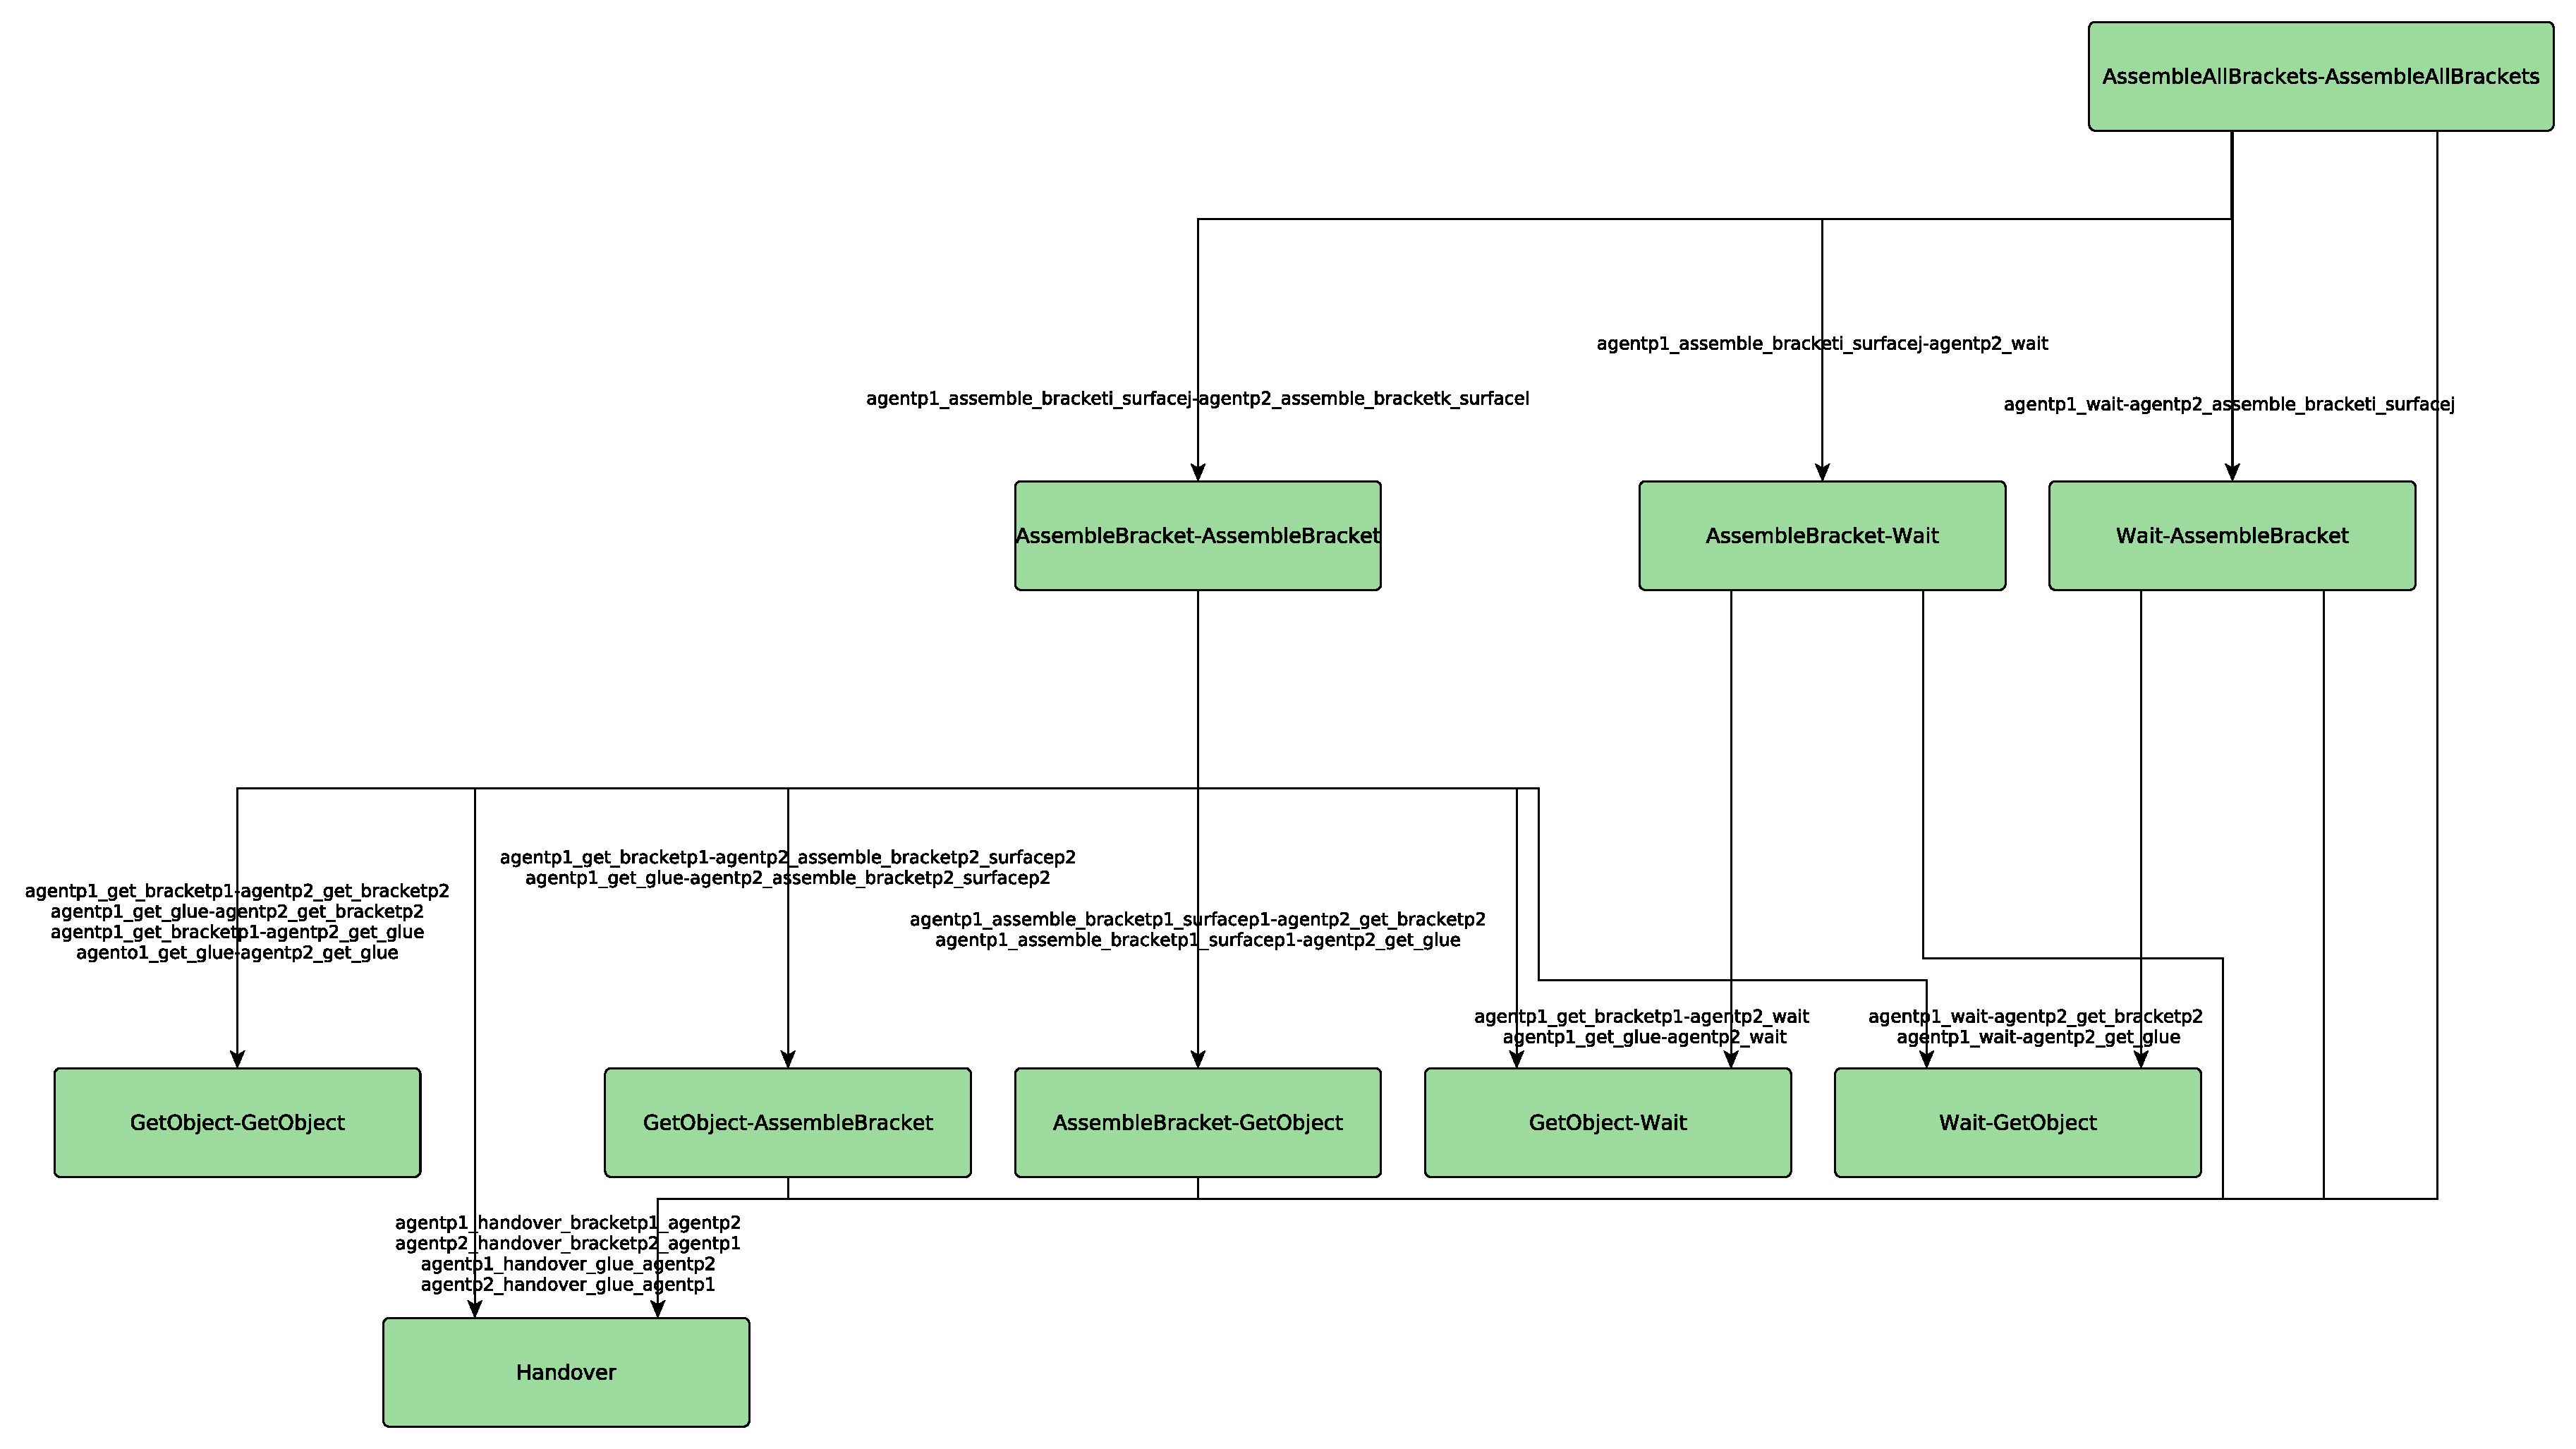
\includegraphics[scale=0.4]{img/coworker/mamdp/scenario_mamdp_architecture.pdf}
	\caption[MAMDP example: MAMDP model]{The image shows the architecture for the MAMDP of the example scenario. The various MAMDPs are represented as rectangles. The arrows show the links between hierarchical modules in the architecture. The label of an arrow shows the macro actions corresponding to the link.}
	\label{fig:mamdp-scenario_mamdp_architecture}
\end{sidewaysfigure}


\subsubsection{AssembleAllBrackets-AssembleAllBrackets}
\begin{itemize}
	\item $name: agent\_assembleallbrackets-agent\_assembleallbrackets$.
	\item		$par: \{agentp1,agentp2\}$.
		\begin{itemize}
			\item $par\_var(agentp1)=agentp1\_isAt$.
			\item $par\_var(agentp2)=agentp2\_isAt$.
		\end{itemize}

		The name of the parameters are changed, adding \textit{pi} at the end, where \textit{i} is the index of the agent. This allows to assign them in an unique way.
	\item $S:\;\{agentp1\_isAt,agentp2\_isAt, bracket1\_isAt,bracket2\_isAt,bracket3\_isAt,\\
	surface1\_status,surface2\_status,surface3\_status\}$. 
		\begin{itemize}
			\item $values(agentp1\_isAt):\{table,surface1,surface2,surface3\}$.
			\item $values(agentp2\_isAt):\{table,surface1,surface2,surface3\}$.
			\item $values(bracketi\_isAt):\{table,surface1,surface2,surface3,agentp1,agentp2\}\; \forall_{i=1}^3$. 
			\item $values(surfacei\_status):\{completed,other\_status\}\;\forall_{i=1}^3$.
		\end{itemize}
		\begin{itemize}
			\item $abstract\_values\_surfacei\_status:$ 
				\begin{itemize}
					\item $none: other\_status$.
					\item $cleaned: other\_status$.
					\item $glued: other\_status$.
				\end{itemize}
		\end{itemize}
		The state set is not very different, simply accounting for the presence of two agents.

	\item $A:\;\{agentp1\_assemble\_bracketi\_surfacej-agentp2\_assemble\_bracketk\_bracketl\}\;\forall_{i=1}^1 \forall_{j=1}^3
	\forall_{k=1}^3 \forall_{l=1}^3 \cup JointActions \cup WaitActions$.
	\item $JointActions=agentpi\_handover\_bracketj\_agentpl \; \forall_{i=1}^2 \; \forall_{j=1}^3 \; \forall_{l=1; l!=i}^3$.
	\item $WaitActions=(agentp1\_assemble\_bracketi\_surfacej-agentp2\_wait \; \cup \\
	 agentp1\_wait-agentp2\_assemble\_bracketi\_surfacej) \; \forall_{i=1}^3 \; \forall_{j=1}^3$.

	The action set is the cartesian product of the actions of the single models, plus actions to exchange brackets, plus actions where only one agent is acting.
	\item $M: A$.
	\item $G:\; \cup_{s:S}\; |\; \forall_{i=1}^3\; surfacei\_status=completed\;\text{AND}\\
	\forall_{i=1}^3\; \exists_{j}\;|\;bracketi\_isAt=surfacej\; \text{AND}\\
	\forall_{i=1}^3\; bracketi\_isAt \neq bracketj\_isAt$.
	\item $S_0:\; \cup_{s:S} \; \exists{1\leq i \leq 3}\; |\; surfacei\_status \neq completed$.

	The starting and goal states are the same as the single-agent model. Since the two models used to create the MAMDP are the same, the intersection and union of the states will be the same.
\end{itemize}


If we would create and solve a new MAMDP for each of these macros, we would create a great quantity of models. Fortunately, as previously said, we can reduce the number of models by creating generic sub-models for a macro that can be used when there are not parameters in common. In this case, we actually need to create a specifc sub-MAMDP for every action of the type \textit{agentp1\_assemble\_bracketi\_surfacej-agentp2\_assemble\_bracketk\_surfacel}, where $i=j$ or $j=l$ (since they would have variables in common), plus a generic sub-MAMDP for all the other cases.

Also, in this example, all the MAMDPs for actions where the same bracket is assembled by two agents on different surfaces would not be created, as their goal states contain incongruent states (since a bracket can not be on two surfaces at the same time and a surface can not contain more than one bracket).

\subsubsection{AssembleBracket-GetObject}
Let us consider the AssembleBracket-GetObject MDP, deeper in the hierarchy. In this case, we will need to create a generic sub-MAMDP, plus specific MDPs for the macros \textit{agentp1\_assemble\_bracketi\_surfacej-agentp2\_get\_bracketi} and \textit{agentp1\_assemble\_bracketi\_surfacej-agentp2\_get\_glue}, since they share resources. We will show parts of this sub-MAMDP.  


\begin{itemize}
	\item $name: agent\_assemblebracket-agent\_getobject$.
	\item		$par: \{agentp1,bracketp1,surfacep1,agentp2,objectp2\}$.
		\begin{itemize}
			\item $par\_var(agentp1)=agentp1\_isAt$.
			\item $par\_var(bracket1)=bracketp1\_isAt$.
			\item $par\_var(surfacep1)=surfacep1\_status$.
			\item $par\_var(agentp2)=agentp2\_isAt$.
			\item $par\_var(object2)=objectp2\_isAt$.
		\end{itemize}

	\item $S:\;\{agentp1\_isAt, bracketp1\_isAt,surfacep1\_status, glue\_isAt, agentp2\_isAt, objectp2\_isAt\}$. 
		\begin{itemize}
			\item $values(agentp1\_isAt):\{surfacep1,other\_location\}$.
			\item $values(bracketp1\_isAt):\{agentp1,surface, other\_location,other\_agent\}$. 
			\item $values(glue\_isAt):\{agentp1,other\_location,other\_agent\}$. 
			\item $values(surfacep1\_status):\{none,cleaned,glued,completed\}$.
			\item $values(agentp2\_isAt):\{table,surface1,surface2,surface3\}$.
			\item $values(objectp2\_isAt):\{table,surface1,surface2,surface3,agentp2,other\_agent\}$. 
		\end{itemize}
		\begin{itemize}
			\item $abstract\_values\_objectp2\_isAt:$ 
				\begin{itemize}
					\item $greg=other\_agent$.
					\item $robot=other\_agent$.
				\end{itemize}	
			\item $abstract\_values\_bracketp1\_isAt:$ 
				\begin{itemize}
					\item $surfacei=other\_location \forall_{i=1}^n$ .
					\item $table=other\_location$.
					\item $greg=other\_agent$.
					\item $robot=other\_agent$.
				\end{itemize}	
			\item $abstract\_values\_glue\_isAt=abstract\_value\_bracketp1\_isAt$ 
			\item $abstract\_values\_agentp1\_isAt:$
				\begin{itemize}
					\item $surfacei=other\_location \forall_{i=1}^n$ .
					\item $table=other\_location$.
				\end{itemize}
		\end{itemize}

	\item $G:\; \cup_{s:S}\; |\; surfacep1\_status=completed\; \text{OR} \; objectp2\_isAt=agentp2$
	\item $S_0:\; \cup_{s:S} \; | \; surfacep1\_status \neq completed \; \text{AND} \; objectp2\_isAt \neq agentp2$

	The goal and starting states of the model are, respectively, the union and intersection of the single models.
\end{itemize}


\subsubsection{Handover}
Finally, to conclude, we show the special handover MAMDP, used for cooperative actions. Since this is a special model, not created by joining two single-agent MDPs, it will not follow the same rules, and instead it will be treated in a similar way as a single agent MDP.

\begin{itemize}
	\item $name: agent1\_handover\_object\_agent2$.
	\item		$par: \{agent1,object,agent2\}$.
		\begin{itemize}
			\item $par\_var(agent1)=agent1\_isAt$.
			\item $par\_var(agent2)=agent2\_isAt$.
			\item $par\_var(object)=object\_isAt$.
		\end{itemize}

	\item $S:\;\{agent1\_isAt, agent2\_isAt, object\_isAt\}$. 
		\begin{itemize}
			\item $values(agent1\_isAt):\{surface1,surface2,surface3,table\}$.
			\item $values(object\_isAt):\{agent1,agent2,other\_location\}$. 
			\item $values(agent2\_isAt):\{surface1,surface2,surface3,table\}$. 
		\end{itemize}
		\begin{itemize}
			\item $abstract\_values\_object2\_isAt:$ 
				\begin{itemize}
					\item $table=other\_location$.
					\item $surface1=other\_location$.
					\item $surface2=other\_location$.
					\item $surface3=other\_location$.
				\end{itemize}	
		\end{itemize}

	\item $A:\;\{agent1\_move\_location-agent2\_move\_location, agent1\_move\_location-agent2\_wait,\\agent1\_wait-agent2\_move\_location, \\ 
	agent1\_give\_object\_agent2-agent2\_receive\_object\_agent1\} \\ \text{where}\; location \in \{table,surface1,surface2,surface3\}$
	\item $G:\; \cup_{s:S} \; | \; object\_isAt=agent2$
	\item $S_0:\; \cup_{s:S} \; | \; object\_isAt=agent1$
\end{itemize}



\section{Enhancing Task Monitoring}
\label{sec:mamdp-plan_monitoring}

In section~\ref{sec:plan_management-plan_monitoring} we introduced the problem of task monitoring. We presented three different problematics: monitoring actions, monitoring tasks, and evaluating human engagement.

We presented a solution only for the problem of monitoring actions. In this section, we propose a strategy to monitor tasks and evaluate the human's engagement, based on the MAMDP model developed in this chapter. We are just starting to investigate this idea, and have not yet completed an implementation.

In general, a MAMDP proposes only the next action in the plan, which is not sufficient to manage plans and ensure synchronism. To deal with this problem, we can compute an horizon of $h$ actions from the MAMDP, building causal links between the nodes to create the stream structure introduced in chapter~\ref{chapter:plan_management}.

\subsection{Evaluating Human Engagement and Monitoring Tasks}
Understanding if a human is engaged in a task is equivalent to infer if its current intention is to achieve the task. As previously said, in section~\ref{subsec:intention-unknown_intentions}, normally, our Intention and Action Recognition module is not able to monitor joint goals. To solve this issue, while performing a shared plan, we create, in the Situation Assessment layer, a new intention for each MAMDP model in the domain. We associate to these intentions the linked MAMDP and the context node \textit{have a shared plan}, which is treated as evidence with a true value. We call these intentions \textit{plan intentions}.

We associate to each known intention a precomputed \textit{expected length}, which is the expected time to accomplish the linked goal.

Using the Intention and Action Recognition module, the robot can infer which is currently the most likely human intention. If the current intention equals the task to monitor, the robot infers that the human is actively working to complete its task.

 We consider the task, and the monitor procedure, as \textit{completed} when the linked MAMDP reaches a \textit{goal state}.

If the human is currently not involved in the monitored task there are three possibilities:
\begin{itemize}
	\item The human has momentarily interrupted the task. This can be inferred if the human is currently involved in another intention, which does not belong to the \textit{plan intentions}, and whose expected length is \textit{short}. In this case, the monitor procedure will not return an error until a predefined \textit{allowed time}.
	\item The human has abandoned the task.  This can be inferred if the human is currently involved in another intention, which does not belong to the \textit{plan intentions}, and whose expected length is \textit{long}. The monitor will return an error. 
	\item The human is performing another task in the shared goal. This can be inferred if the human is currently involved in another intention, which belongs to the \textit{plan intentions}. In this case the monitor will return an error. 
\end{itemize}




 
